% Validation section should include: 
% Data/MC Agreement after precuts on all important variables
% Sideband Checks
% Corsika In-time vs BNB-ext
% Future Validation Studies

\section{Validation}

\subsection{Simulation/Data Comparisons}
In this section we will validate the background rejection cuts described in Section \ref{sec:bkg}. In particular, for each variable, we will show:
\begin{itemize}
\item the integral-normalized Monte Carlo distributions for the signal ($\nu_{e}$ CC0$\pi$-Np events), the cosmogenic background (cosmic, cosmic contaminated, and cosmic in-time), and the neutrino background ($\nu_{e}$ CC, beam intrinsic $\nu_{\mu}$, beam intrinsic NC, and dirt);

\item the POT-normalized Monte Carlo and data distributions, to verify the agreement of the simulation with the collected data.
\end{itemize}

\begin{description}
\item[Most energetic shower $E > 50~\mathrm{MeV}$.] The integral-normalized distributions in Figure \ref{fig:showere_integral} show that a large fraction of the cosmogenic and neutrino backgrounds have very low-energetic showers, while the signal component is almost constant. Figure \ref{fig:showere_pot} shows a good data/Monte Carlo agreement for this variable ($\chi^2 / \mathrm{n.d.f.} = 1.17$).

\begin{figure}[htbp]
\centering
  \begin{subfigure}{0.45\textwidth}
    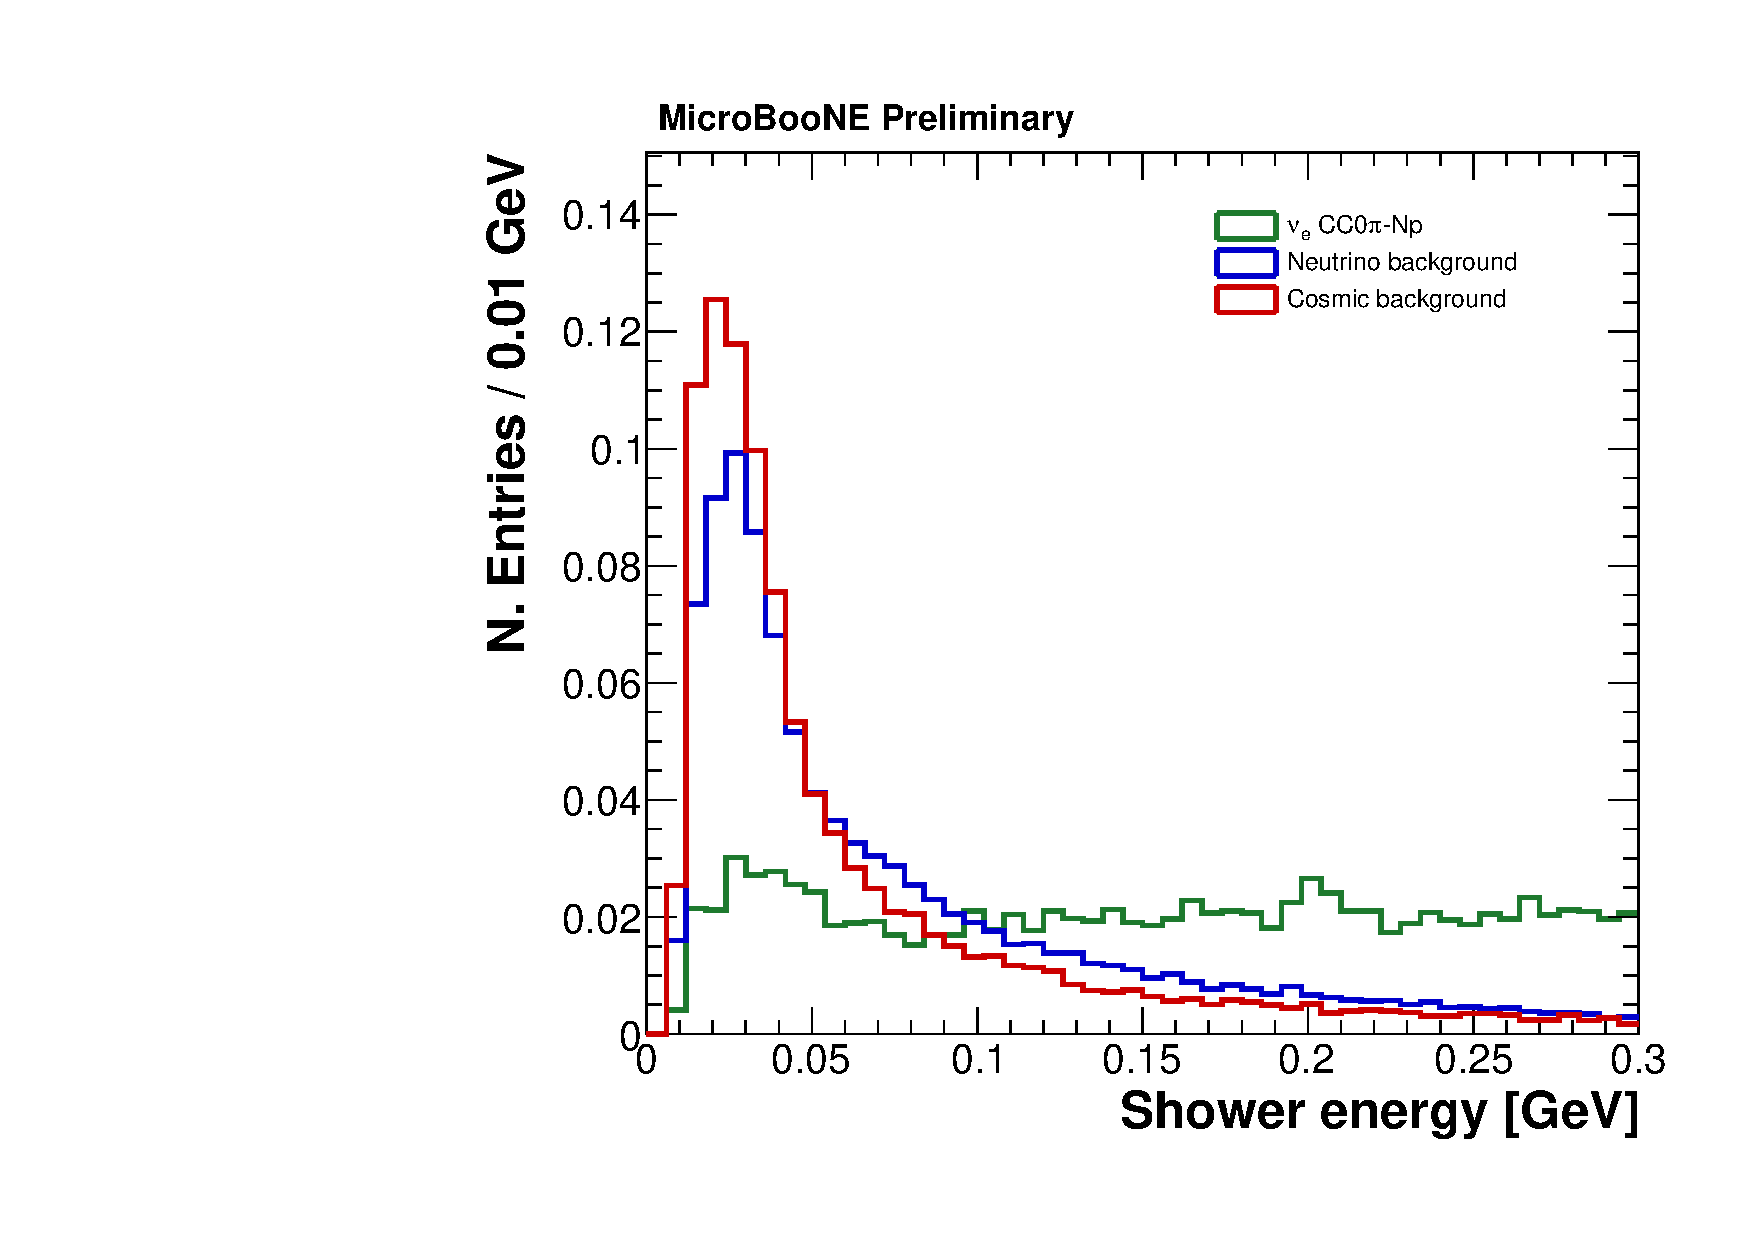
\includegraphics[width=\linewidth]{figures/h_shower_energy_norm.pdf}
    \caption{Integral normalized.} \label{fig:showere_integral}
  \end{subfigure}
    \begin{subfigure}{0.45\textwidth}
    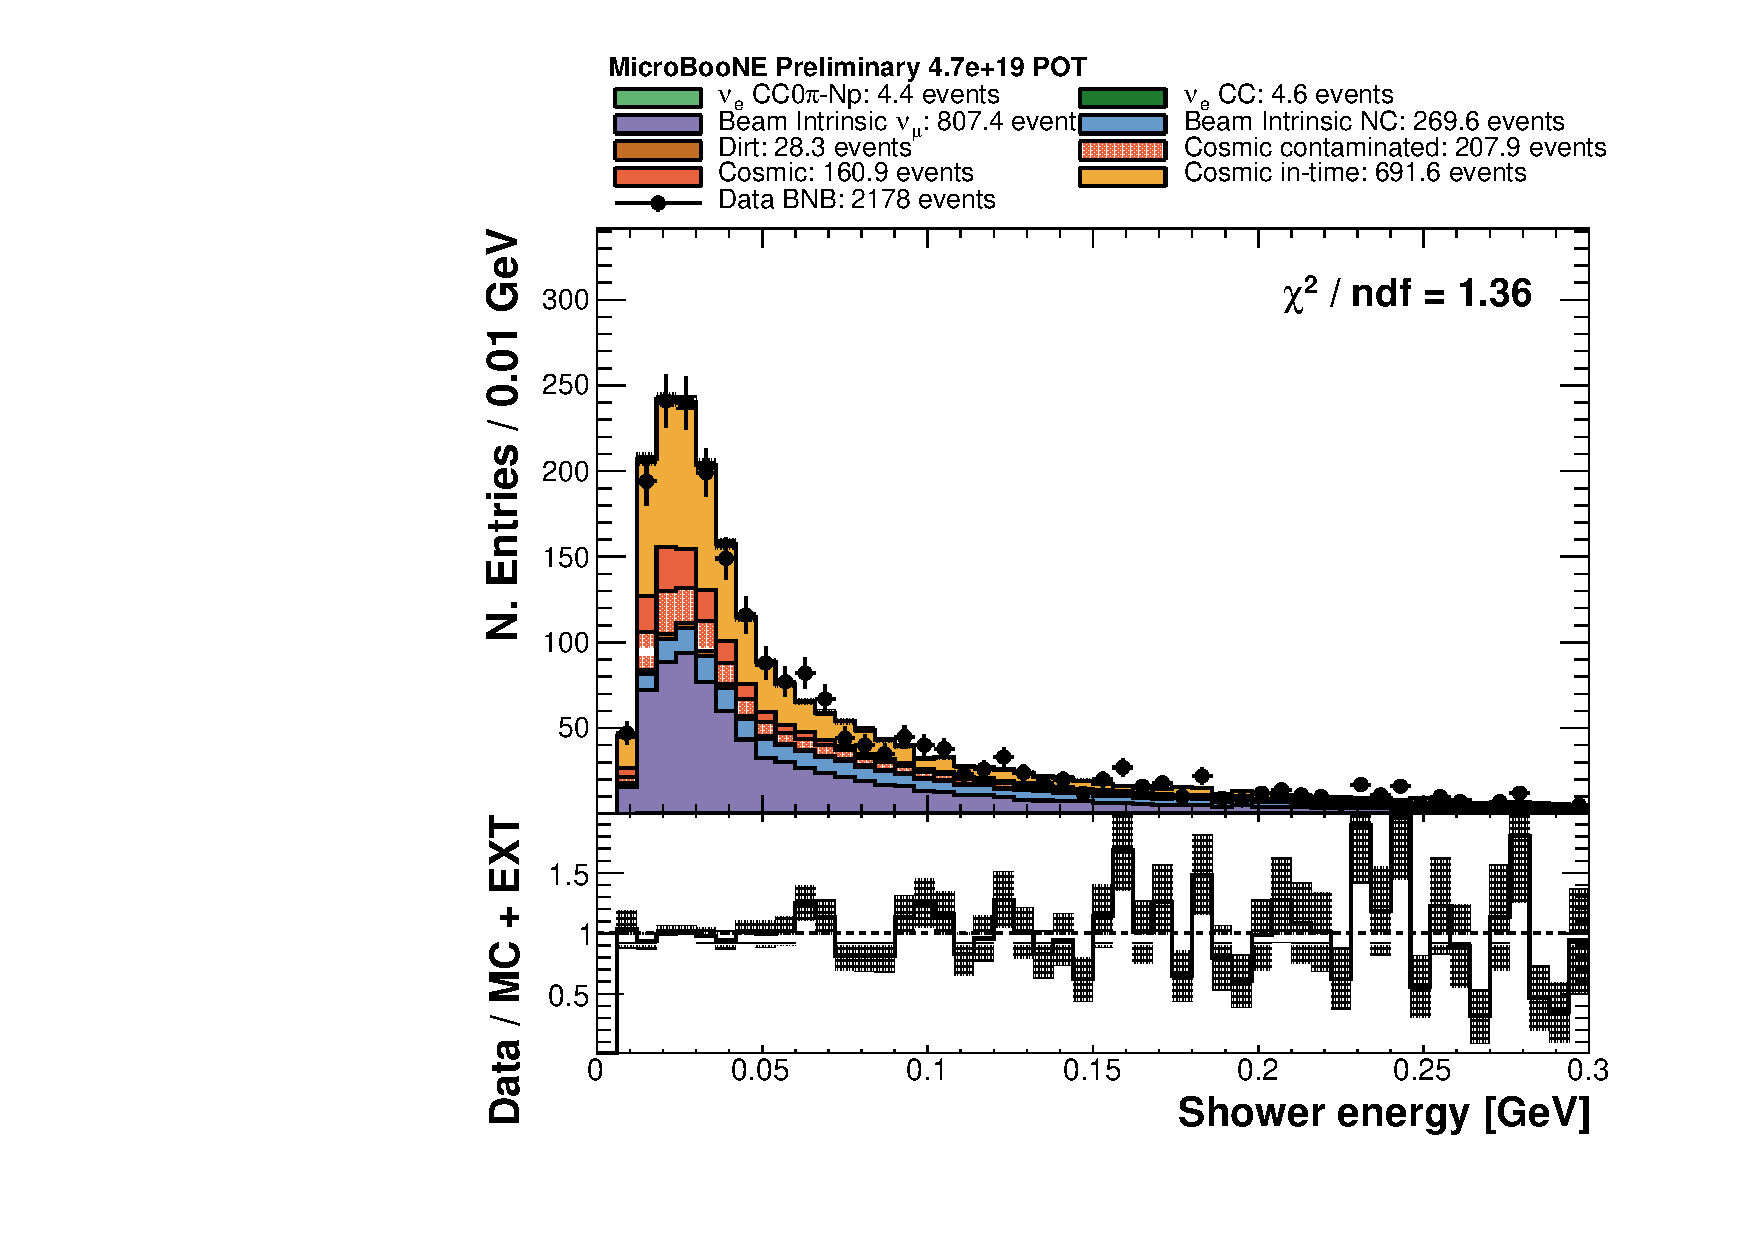
\includegraphics[width=\linewidth]{figures/h_shower_energy.pdf}
    \caption{POT normalized.} \label{fig:showere_pot}
  \end{subfigure}
  \caption{Integral and POT normalized distributions of the energy of the most energetic shower.}
\end{figure}

\item[Most energetic shower $1~\mathrm{MeV/cm} < dE/dx <3.2~\mathrm{MeV/cm}$.] Figure \ref{fig:dedx_integral} shows that the signal distribution is peaked around 2 MeV/cm, as expected. The beam intrinsic NC component has a second peak around 4 MeV/cm, mainly caused by $\pi^0\rightarrow2\gamma$ decays. The POT-normalized plot (Figure \ref{fig:dedx_pot}) shows a very good data/Monte Carlo agreement ($\chi^2 / \mathrm{n.d.f.} = 0.87$).

\begin{figure}[htbp]
\centering
  \begin{subfigure}{0.45\textwidth}
    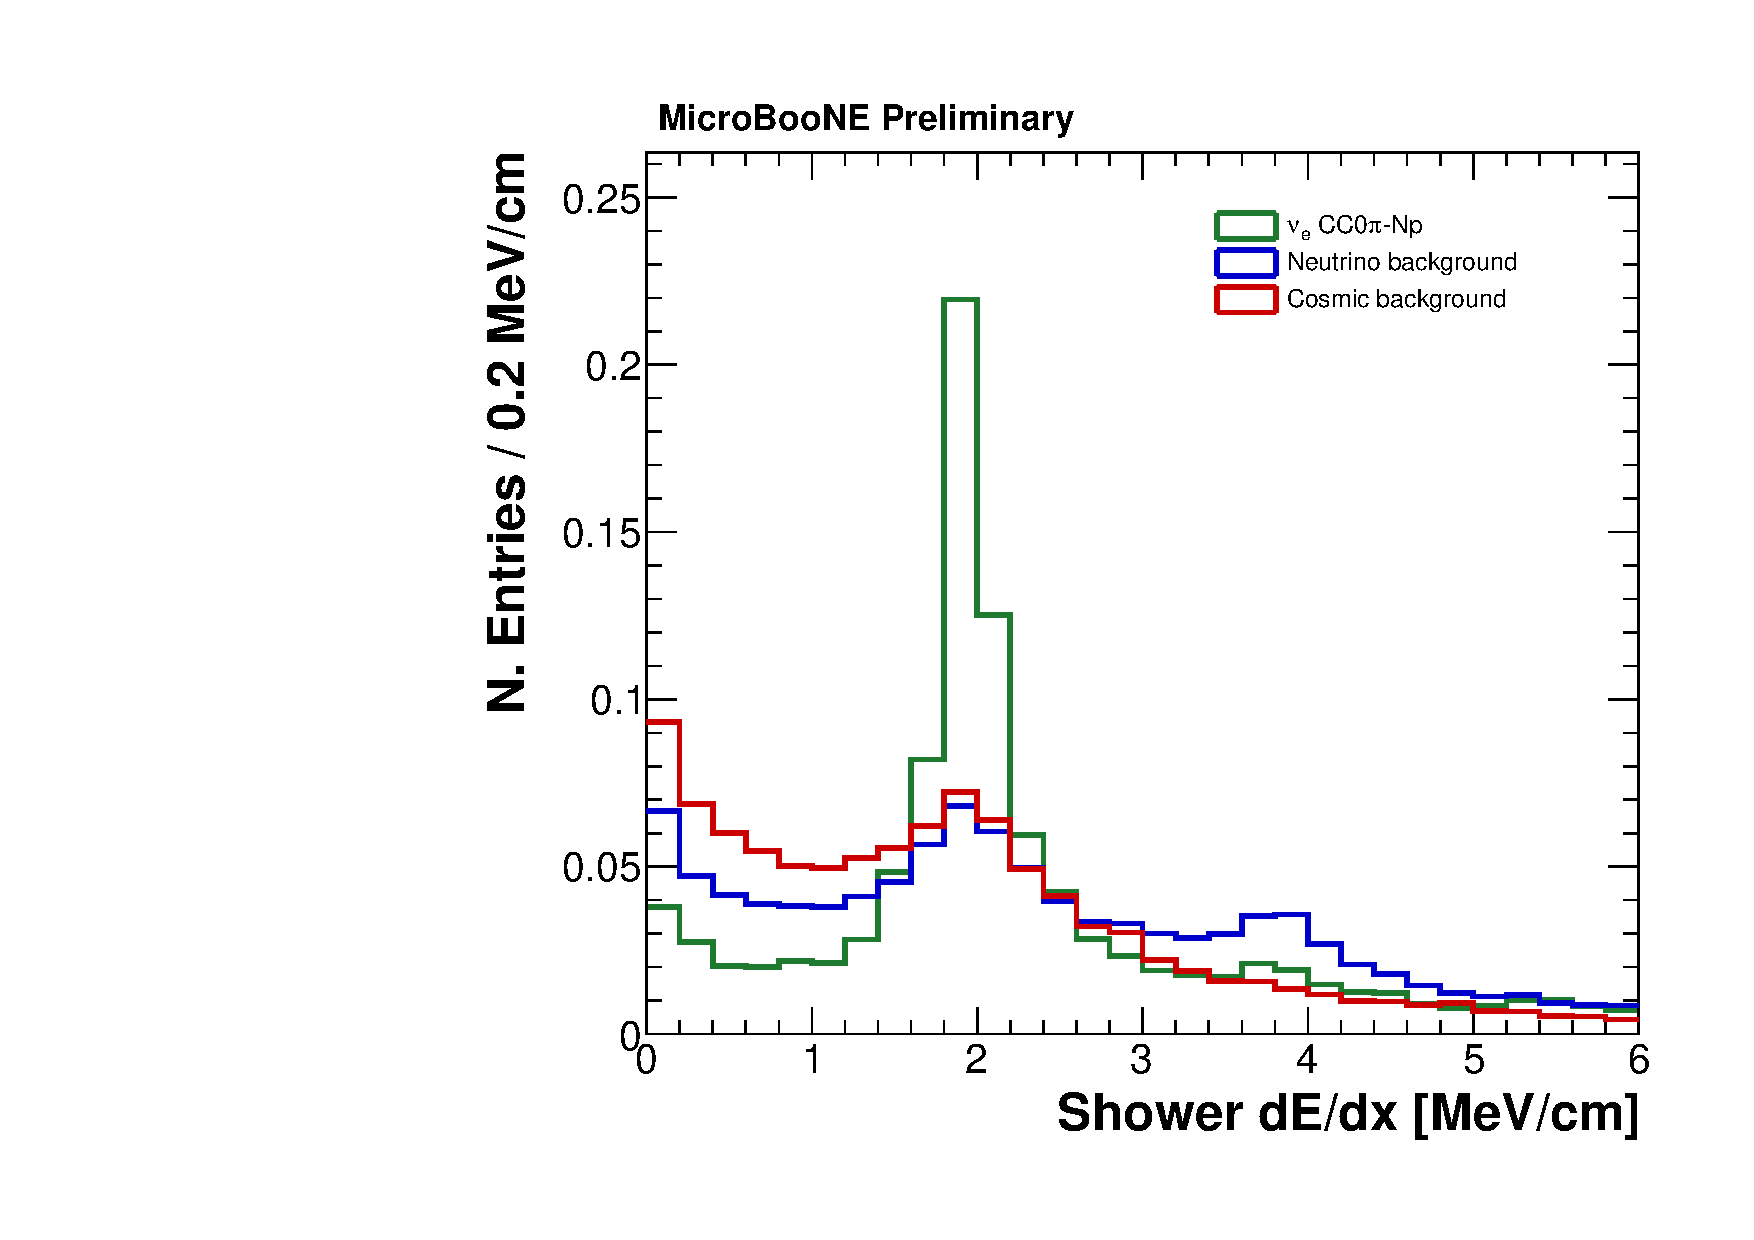
\includegraphics[width=\linewidth]{figures/h_dedx_norm.pdf}
    \caption{Integral normalized.} \label{fig:dedx_integral}
  \end{subfigure}
    \begin{subfigure}{0.45\textwidth}
    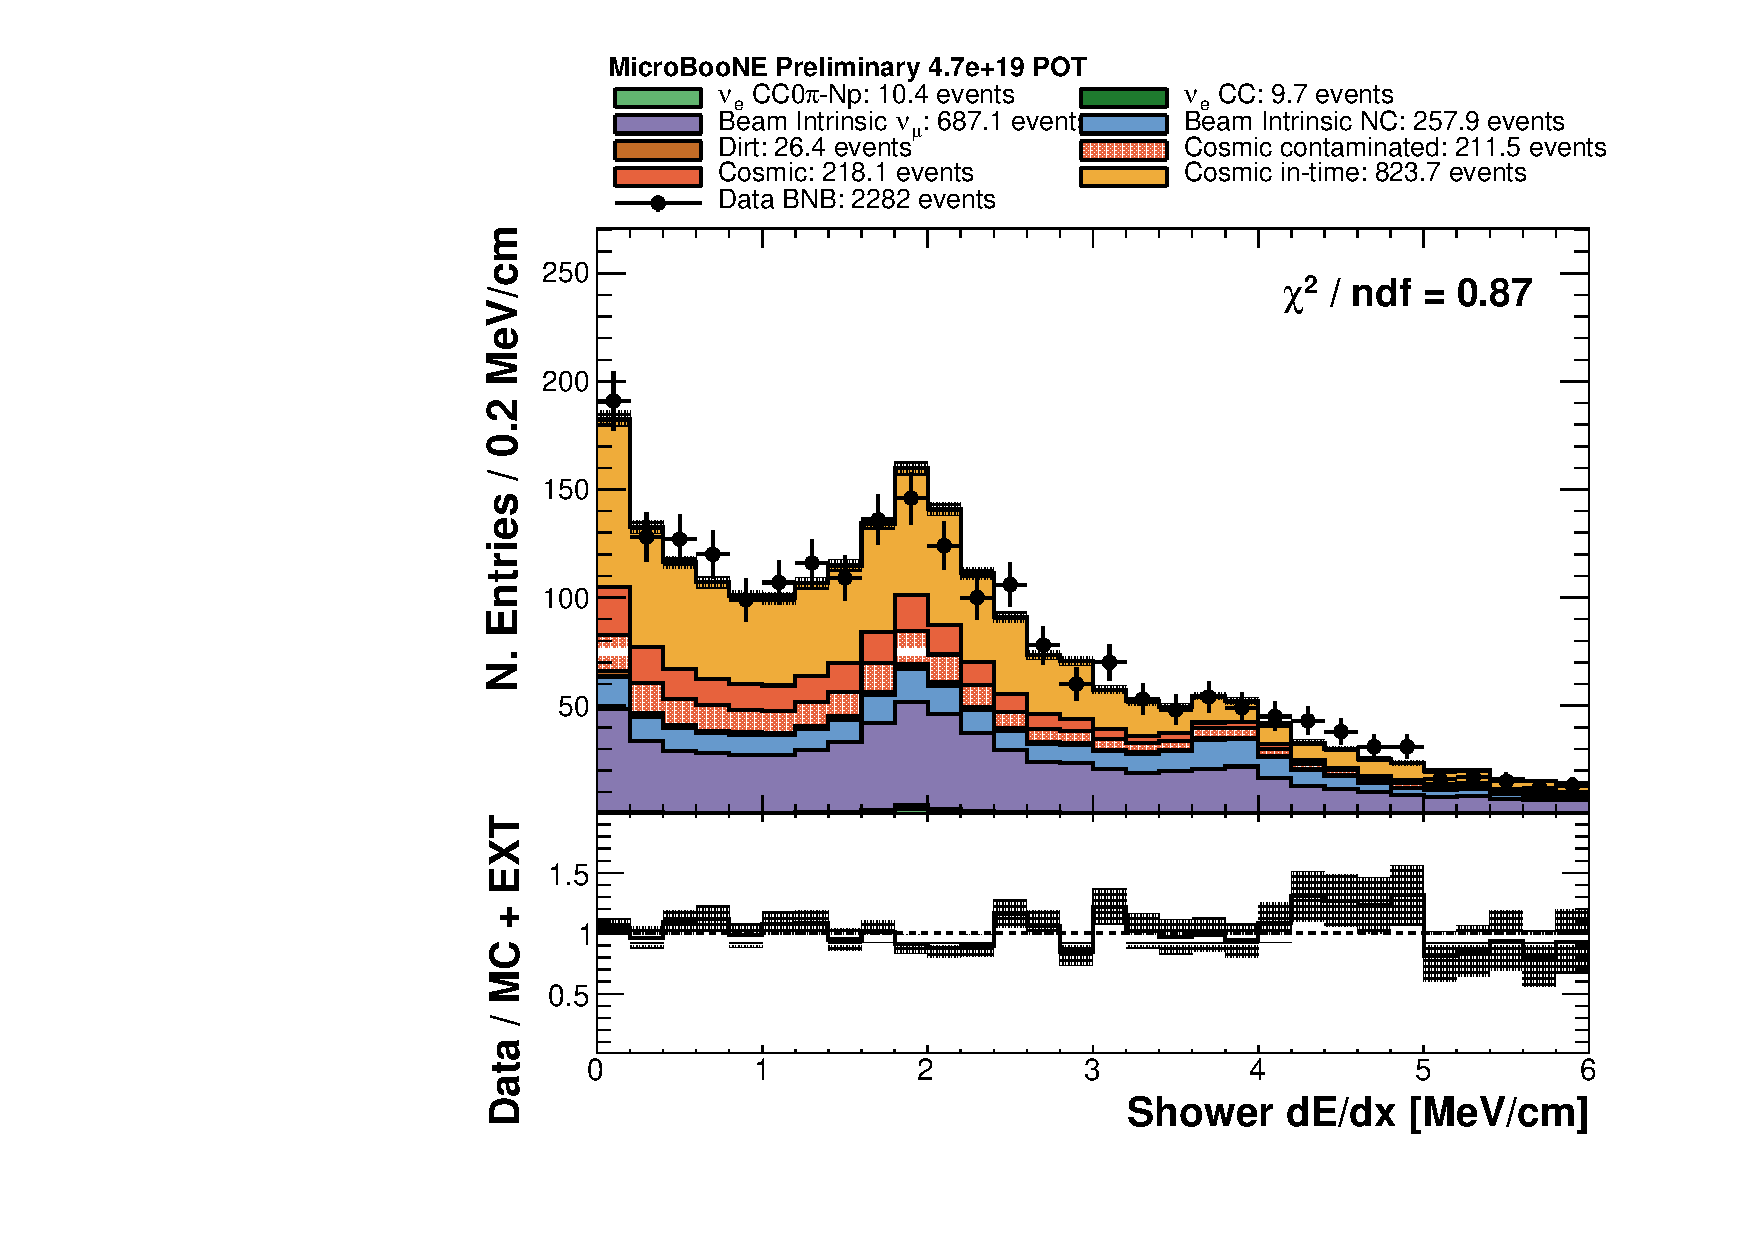
\includegraphics[width=\linewidth]{figures/h_dedx.pdf}
    \caption{POT normalized.} \label{fig:dedx_pot}
  \end{subfigure}
  \caption{Integral and POT normalized distributions of the $dE/dx$ of the most energetic shower.}
\end{figure}

\item[Track distance $d_{t} < 3$~cm.] Figure \ref{fig:track_norm} shows that the distributions of the distance between the reconstructed tracks and the reconstructed neutrino vertex for signal and background are very similar. The cut $d_{t} < 3$~cm, then, mainly ensures that the event is well reconstructed. The data/Monte Carlo agreement in Figure \ref{fig:track_pot} is good, except for the first bin ($0~\mathrm{cm} < d_{t} < 0.5~\mathrm{cm}$), where we have a 10\% more Monte Carlo events than data. This small discrepancy can be explained by a slightly better vertex resolution in the simulation compared to data.

\begin{figure}[htbp]
\centering
  \begin{subfigure}{0.45\textwidth}
    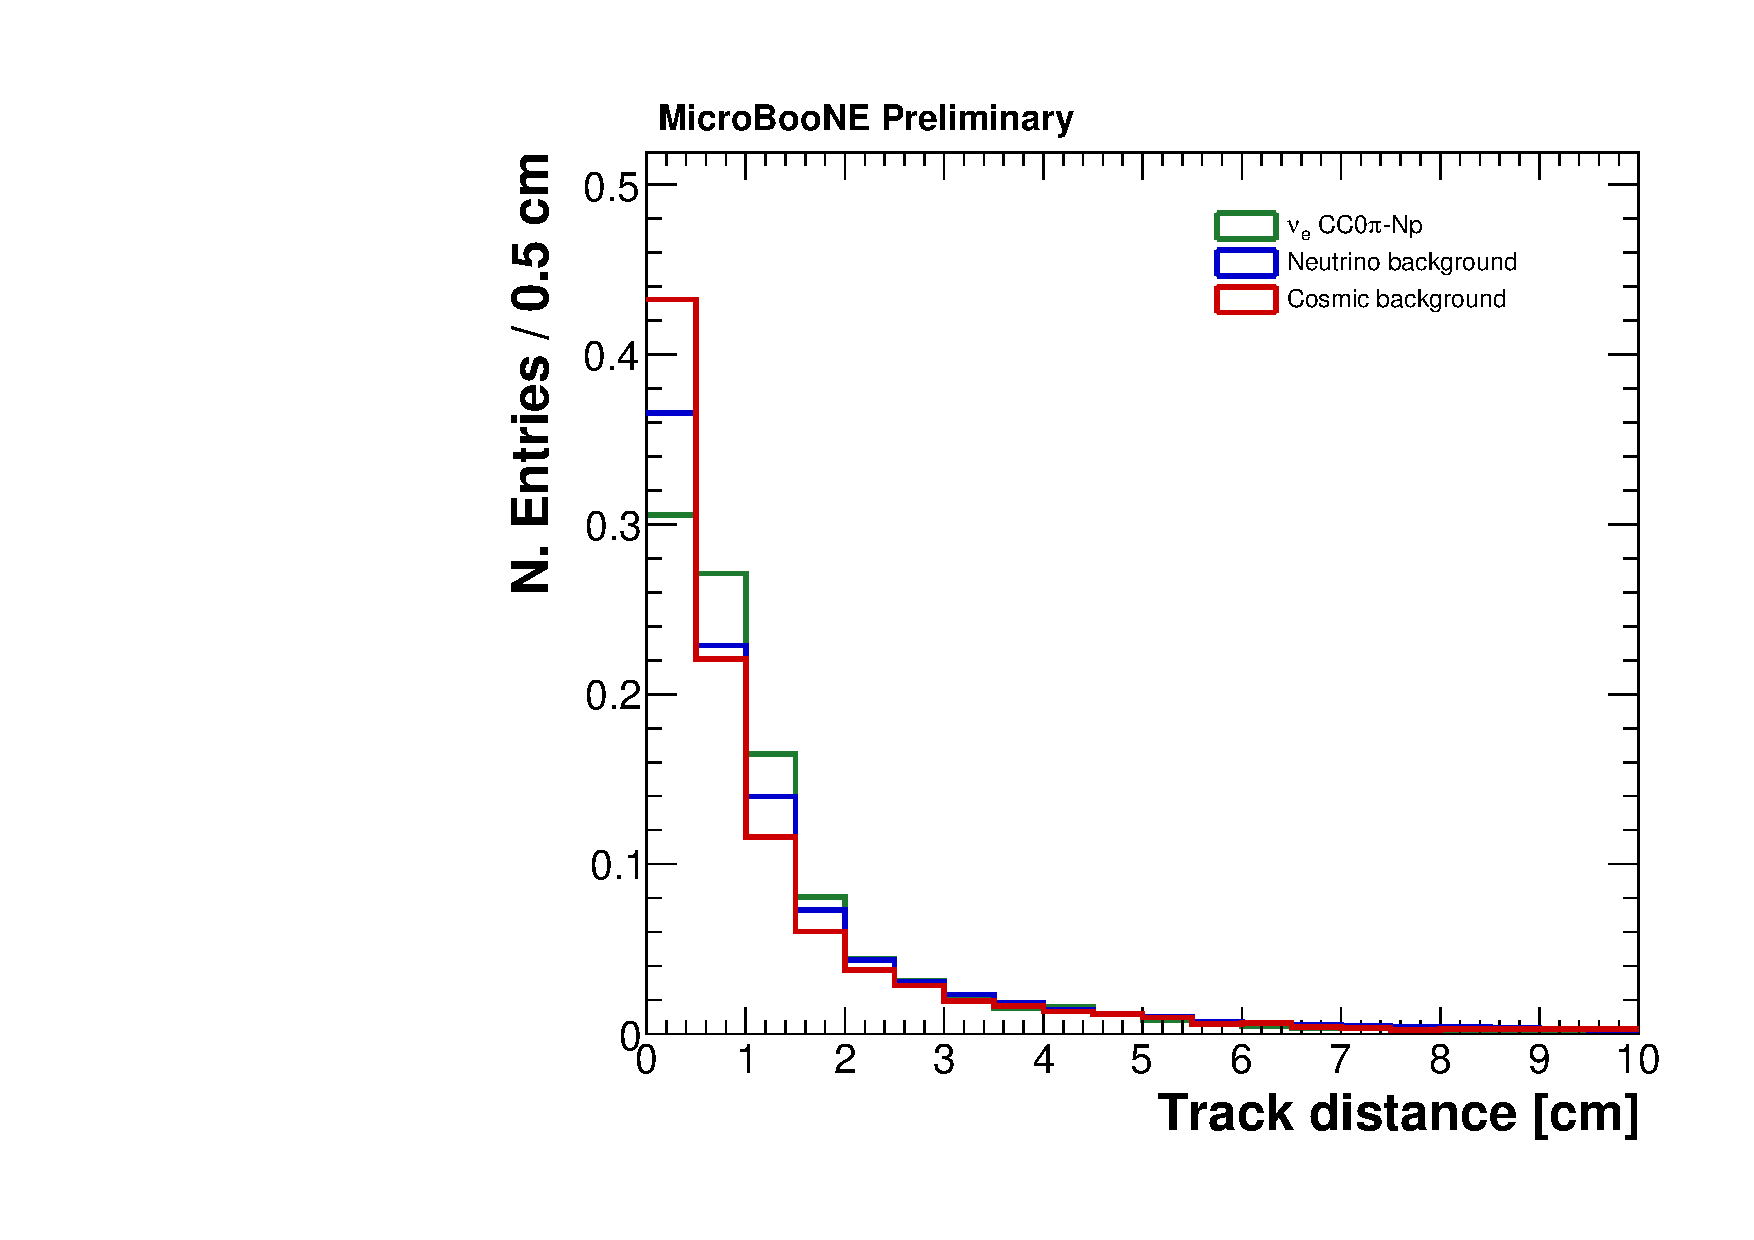
\includegraphics[width=\linewidth]{figures/h_track_distance_norm.pdf}
    \caption{Integral normalized.} \label{fig:track_norm}
  \end{subfigure}
    \begin{subfigure}{0.45\textwidth}
    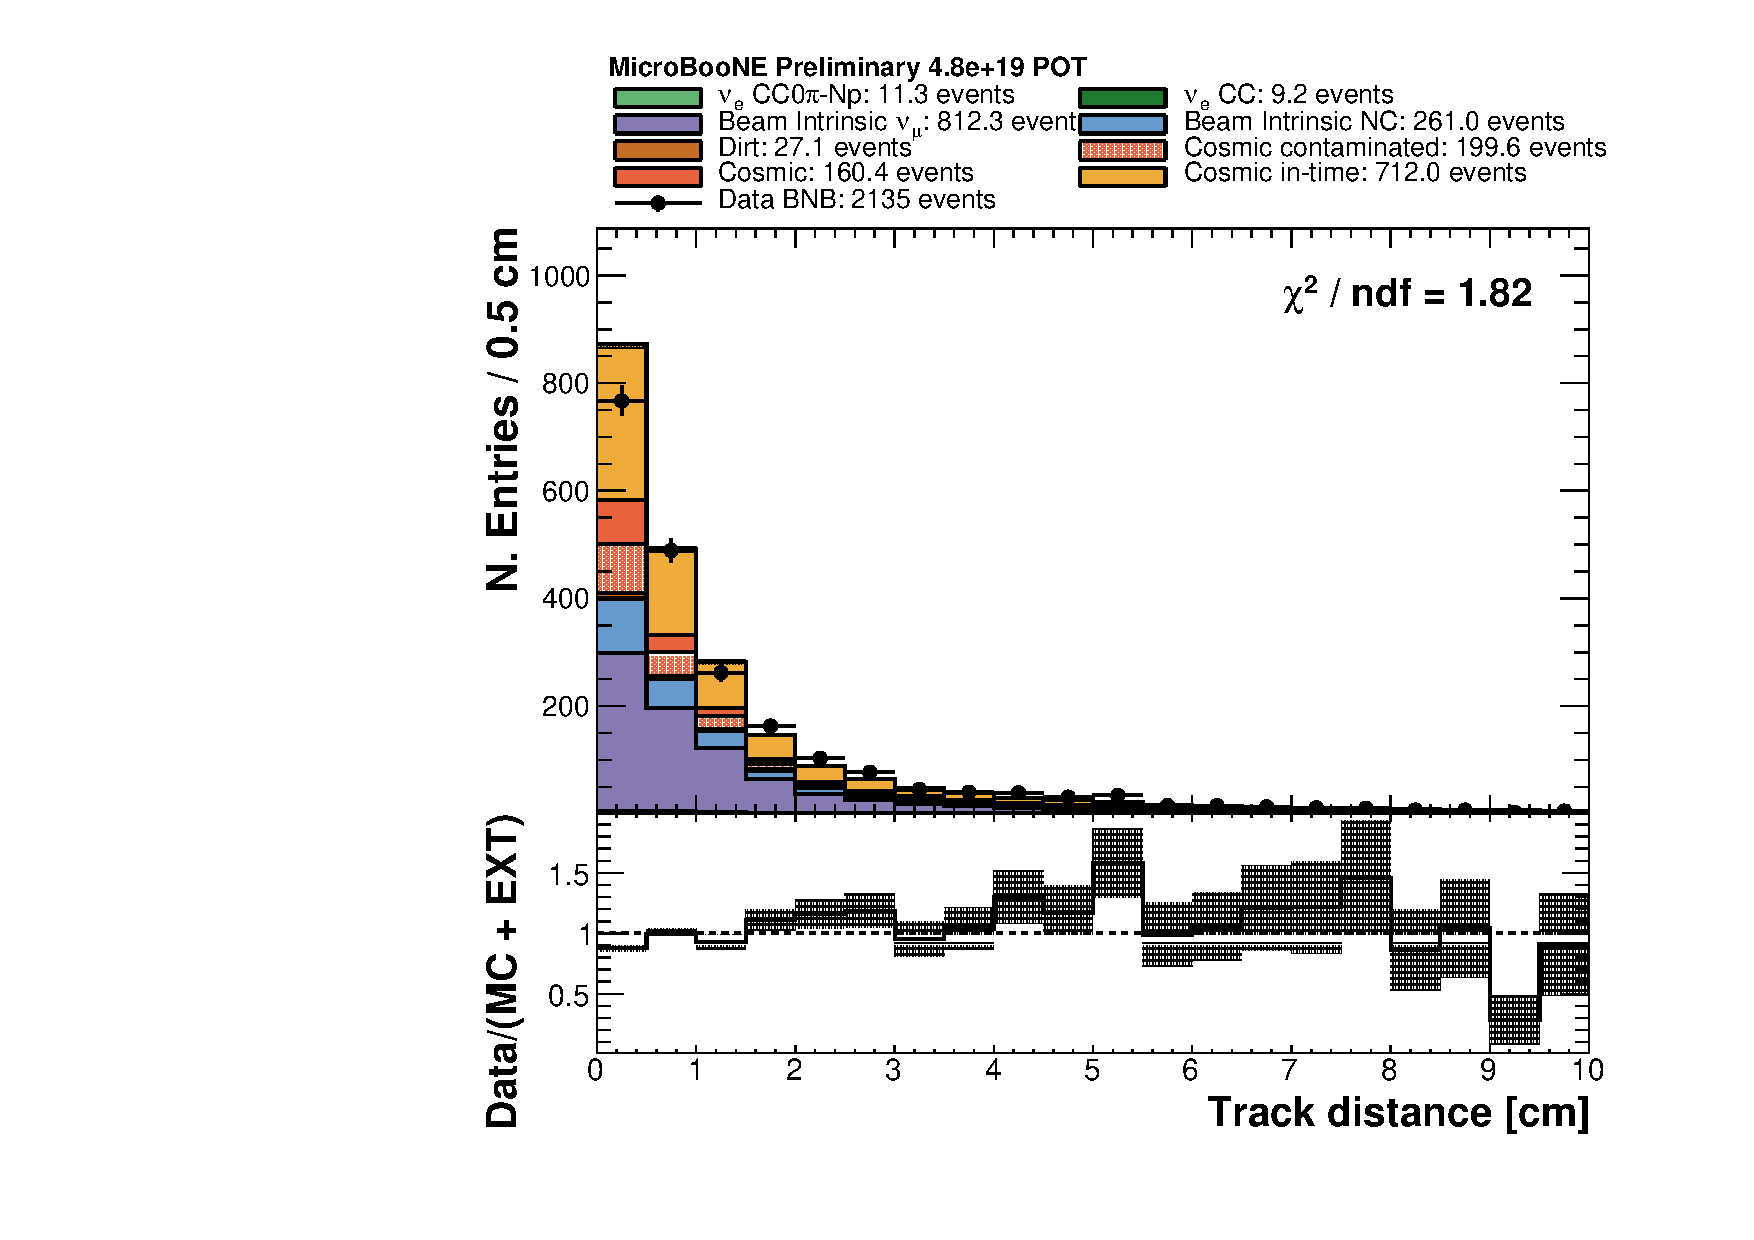
\includegraphics[width=\linewidth]{figures/h_track_distance.pdf}
    \caption{POT normalized.} \label{fig:track_pot}
  \end{subfigure}
  \caption{Integral and POT normalized distributions of the distance between each reconstructed track and the reconstructed neutrino vertex.}
\end{figure}

\item[Proton track BDT score $> -0.12$.] Figure \ref{fig:bdt_norm} shows the BDT score for the tracks in background and signal events, trained with the procedure described in Section \ref{sec:protbdt}. The cut at $-0.12$ allows to remove events with muon-like tracks. The data/Monte Carlo agreement shown in figure \ref{fig:bdt_pot} is good both in the signal region (high score) and in the background region (low score). The peak at -1 is caused by events with invalid $dQ/dx$ values (e.g. because of wrong vertex reconstruction).

\begin{figure}[htbp]
\centering
  \begin{subfigure}{0.45\textwidth}
    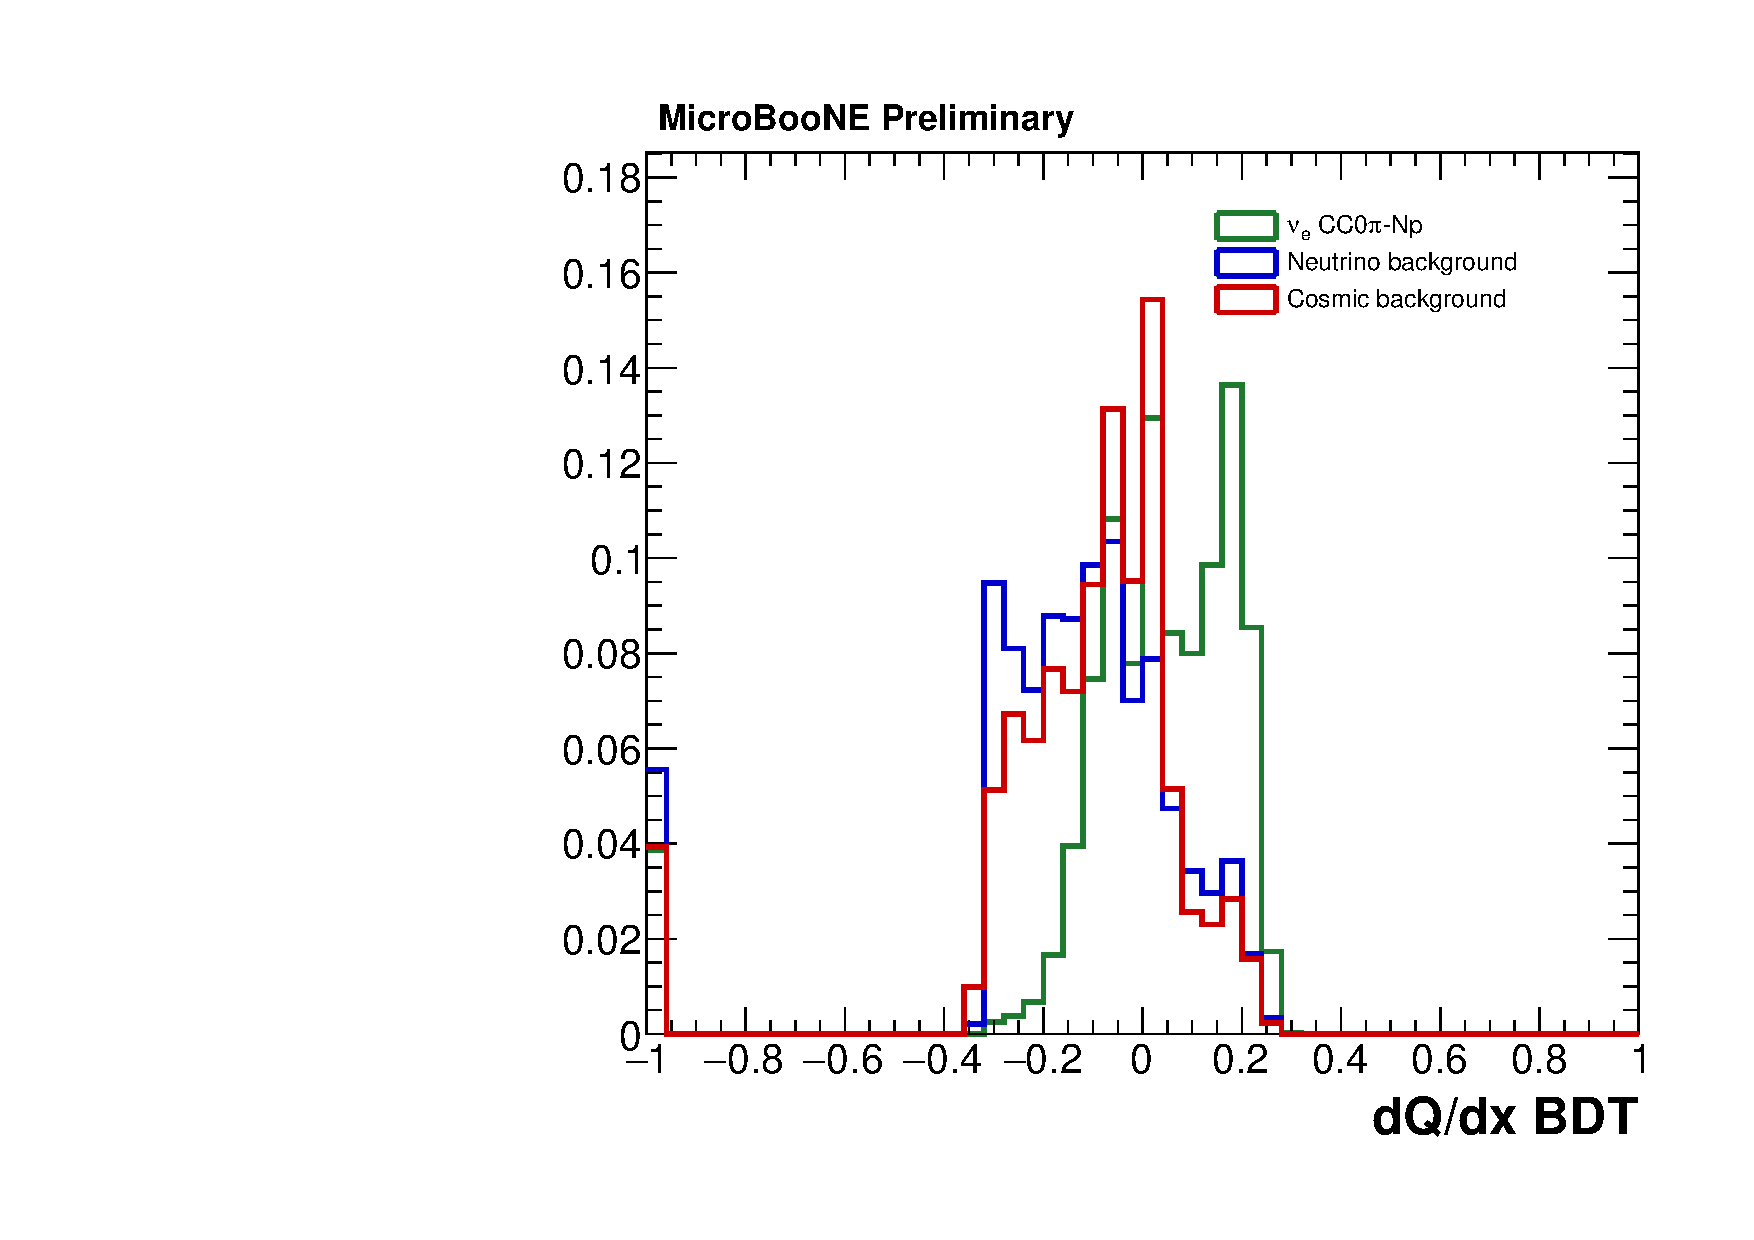
\includegraphics[width=\linewidth]{figures/h_dqdx_bdt_norm.pdf}
    \caption{Integral normalized.} \label{fig:bdt_norm}
  \end{subfigure}
    \begin{subfigure}{0.45\textwidth}
    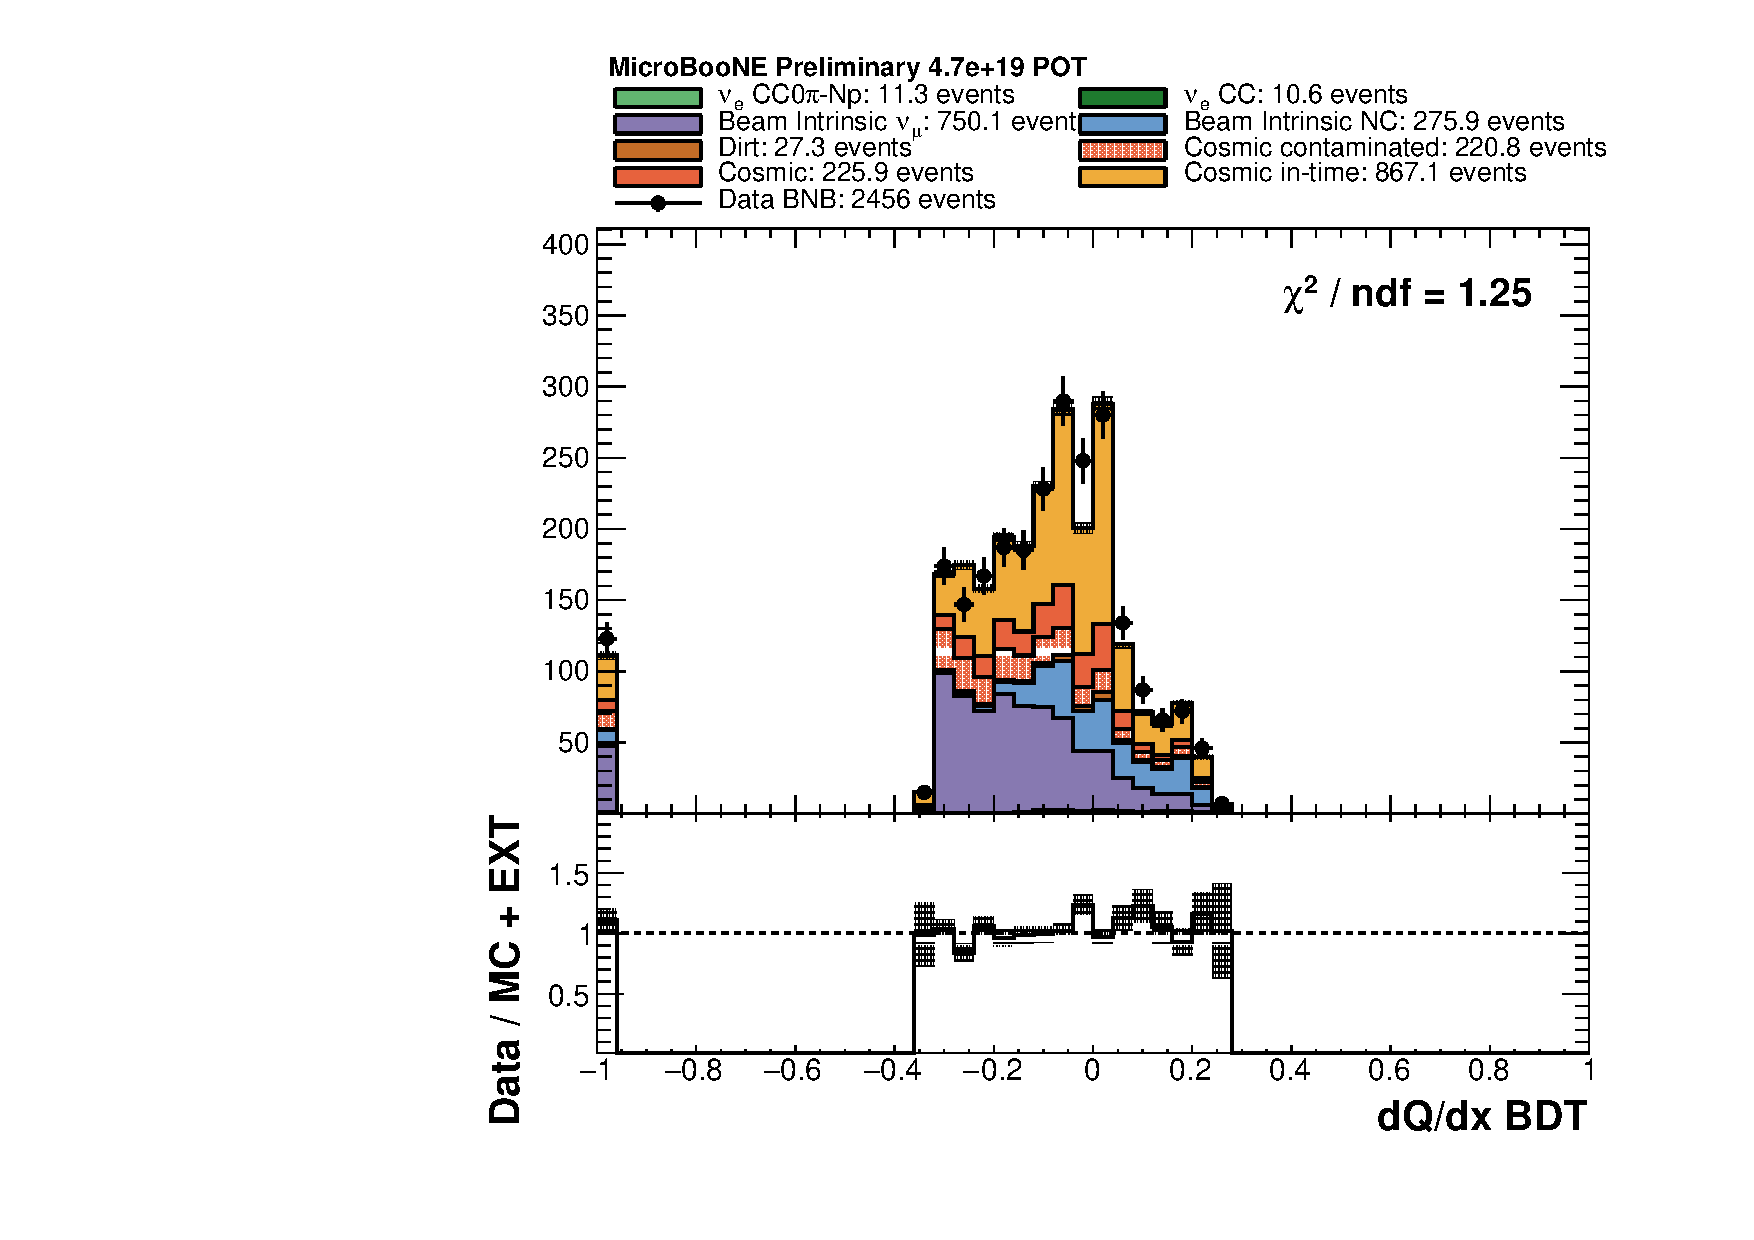
\includegraphics[width=\linewidth]{figures/h_dqdx_bdt.pdf}
    \caption{POT normalized.} \label{fig:bdt_pot}
  \end{subfigure}
  \caption{Integral and POT normalized distributions of the BDT score of the reconstructed tracks.}
\end{figure}


\item[Track-shower angle $\mathrm{cos}\theta > -0.9$]. Figure \ref{fig:angle_integral} shows that there are, in proportion, more background events for events with a high angle between the most proton-like track and the most energetic shower. This cut allows to reject these events while also ensuring that the signal events are well-reconstructed. In fact, signal events with $\mathrm{cos}\theta \approx 1$ have almost always an electron shower reconstructed as a track-like object in the first part. The agreement shown in Figure \ref{fig:angle_pot} is good.

\begin{figure}[htbp]
\centering
  \begin{subfigure}{0.45\textwidth}
    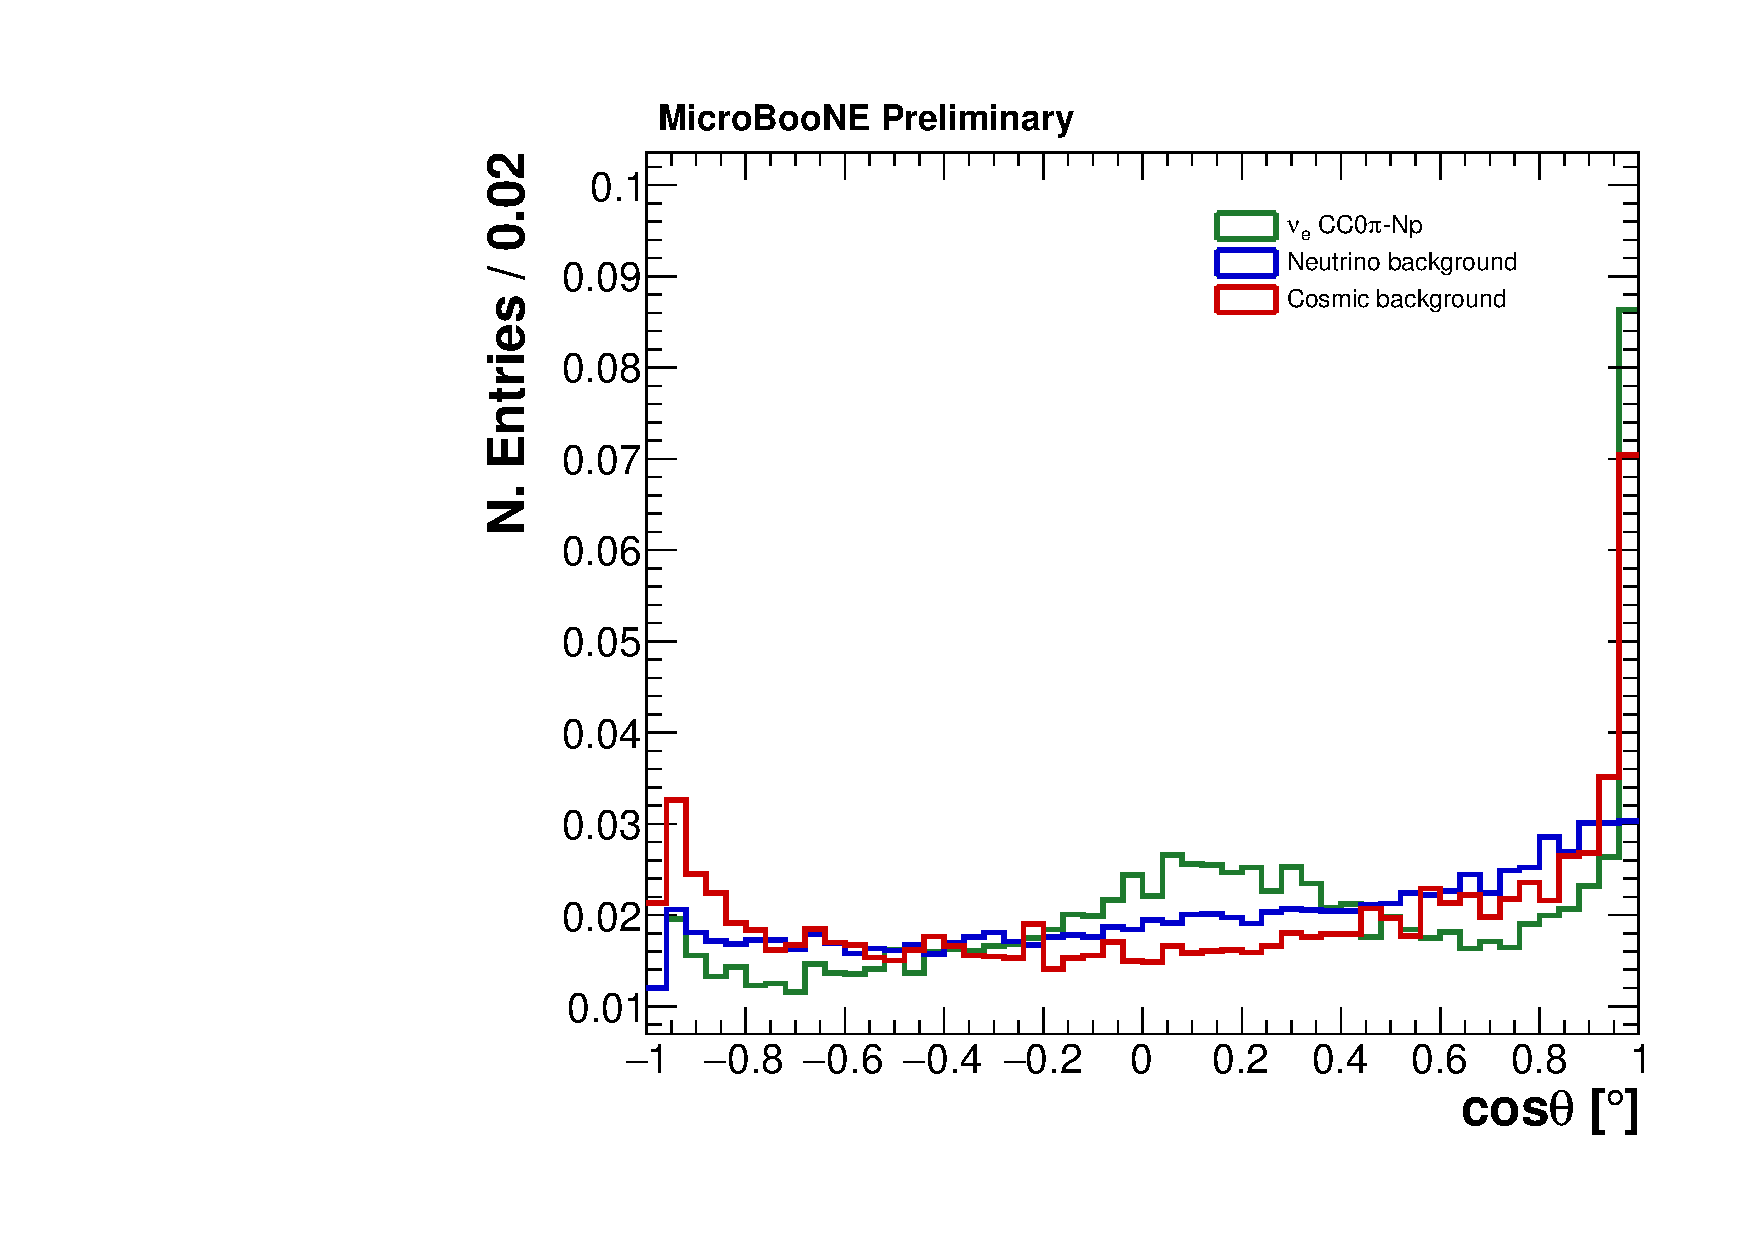
\includegraphics[width=\linewidth]{figures/h_track_shower_angle_norm.pdf}
    \caption{Integral normalized.} \label{fig:angle_integral}
  \end{subfigure}
    \begin{subfigure}{0.45\textwidth}
    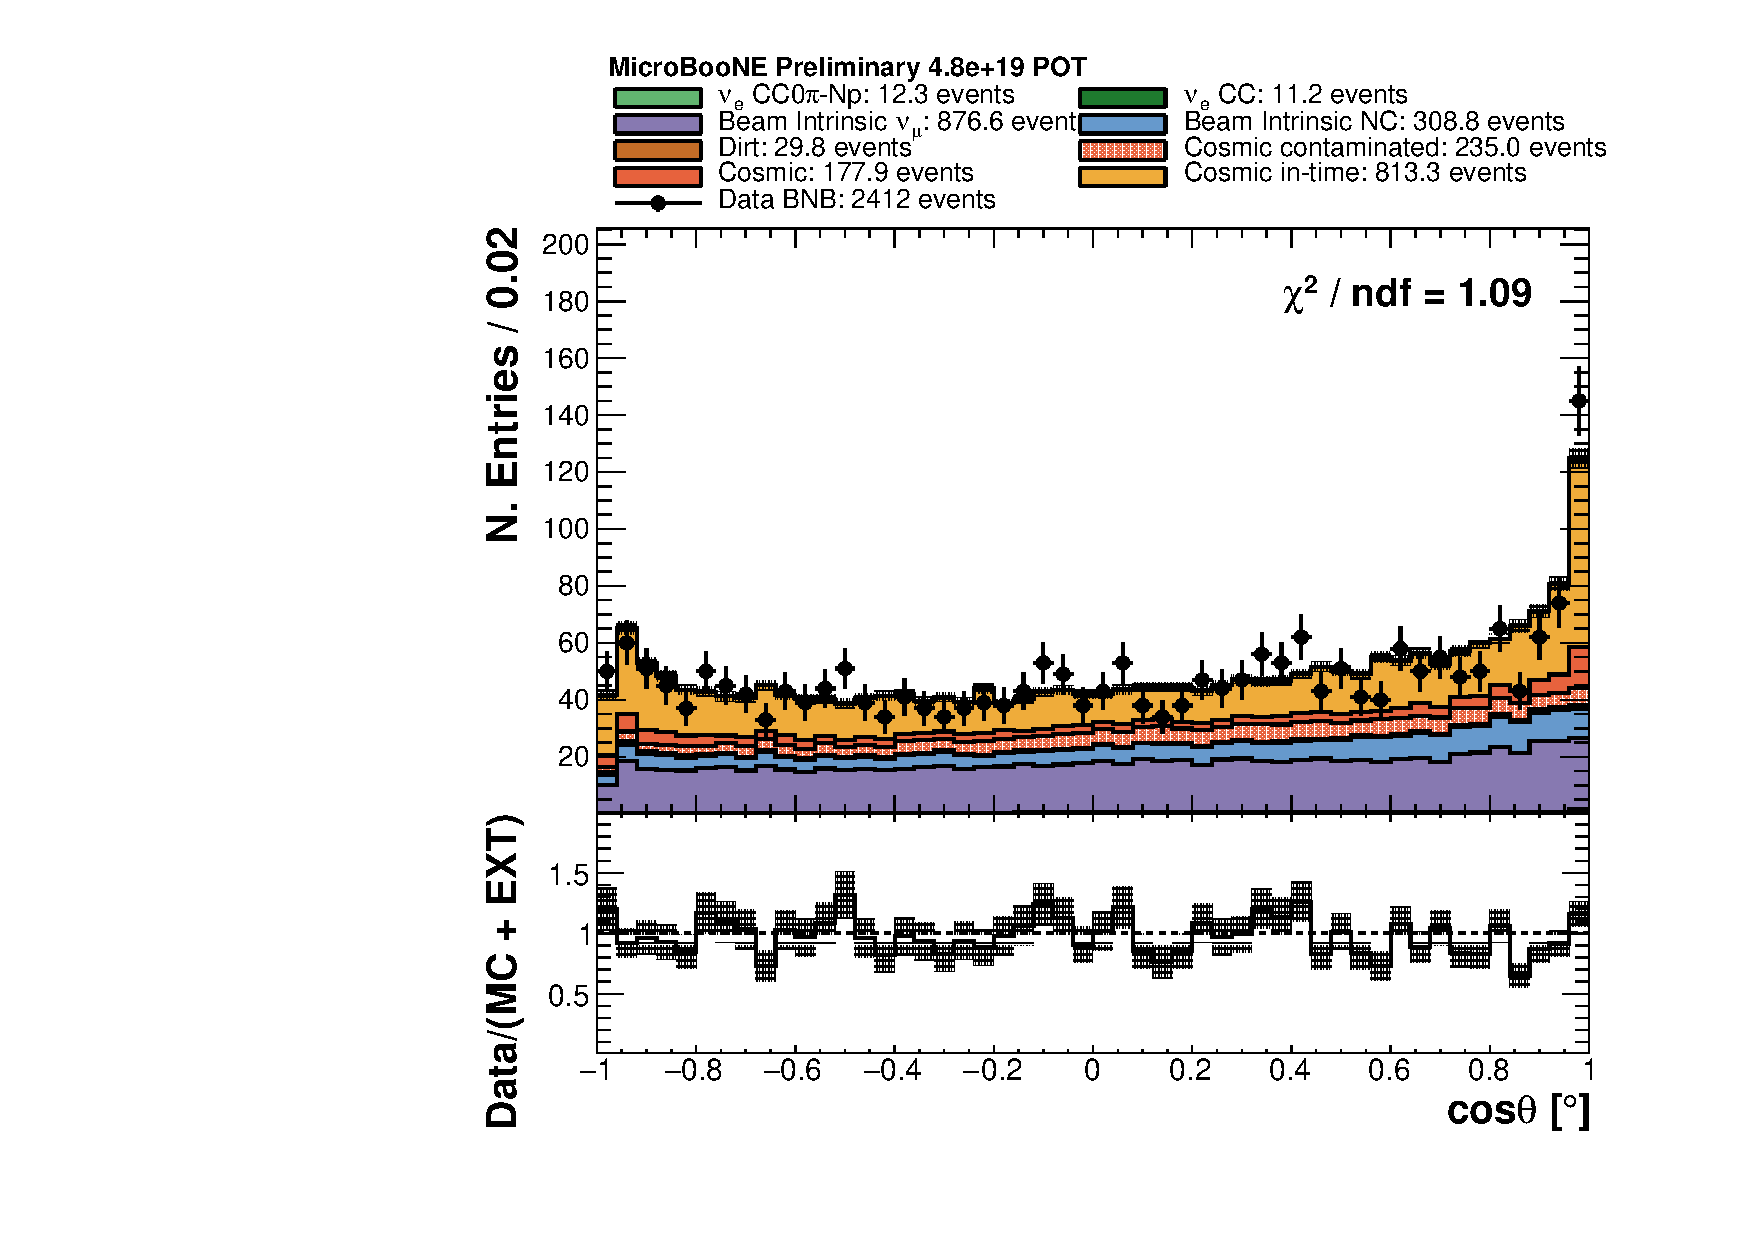
\includegraphics[width=\linewidth]{figures/h_track_shower_angle.pdf}
    \caption{POT normalized.} \label{fig:angle_pot}
  \end{subfigure}
  \caption{Integral and POT normalized distributions of the angle between the most proton-like track and the most energetic shower.}
\end{figure}

\item[Most energetic shower opening angle $1^{\circ} < \theta < 20^{\circ}$]. The distributions of the opening angle $\theta$ of the most energetic shower for neutrino and cosmic background events have a larger tail than the signal events, as shown in figure \ref{fig:open_integral}. The cut $1^{\circ} < \theta < 20^{\circ}$ helps rejecting some background events, while removing only a small fraction of mainly high-energy signal events. Figure \ref{fig:open_pot} shows a good data/Monte Carlo agreement.

\begin{figure}[htbp]
\centering
  \begin{subfigure}{0.45\textwidth}
    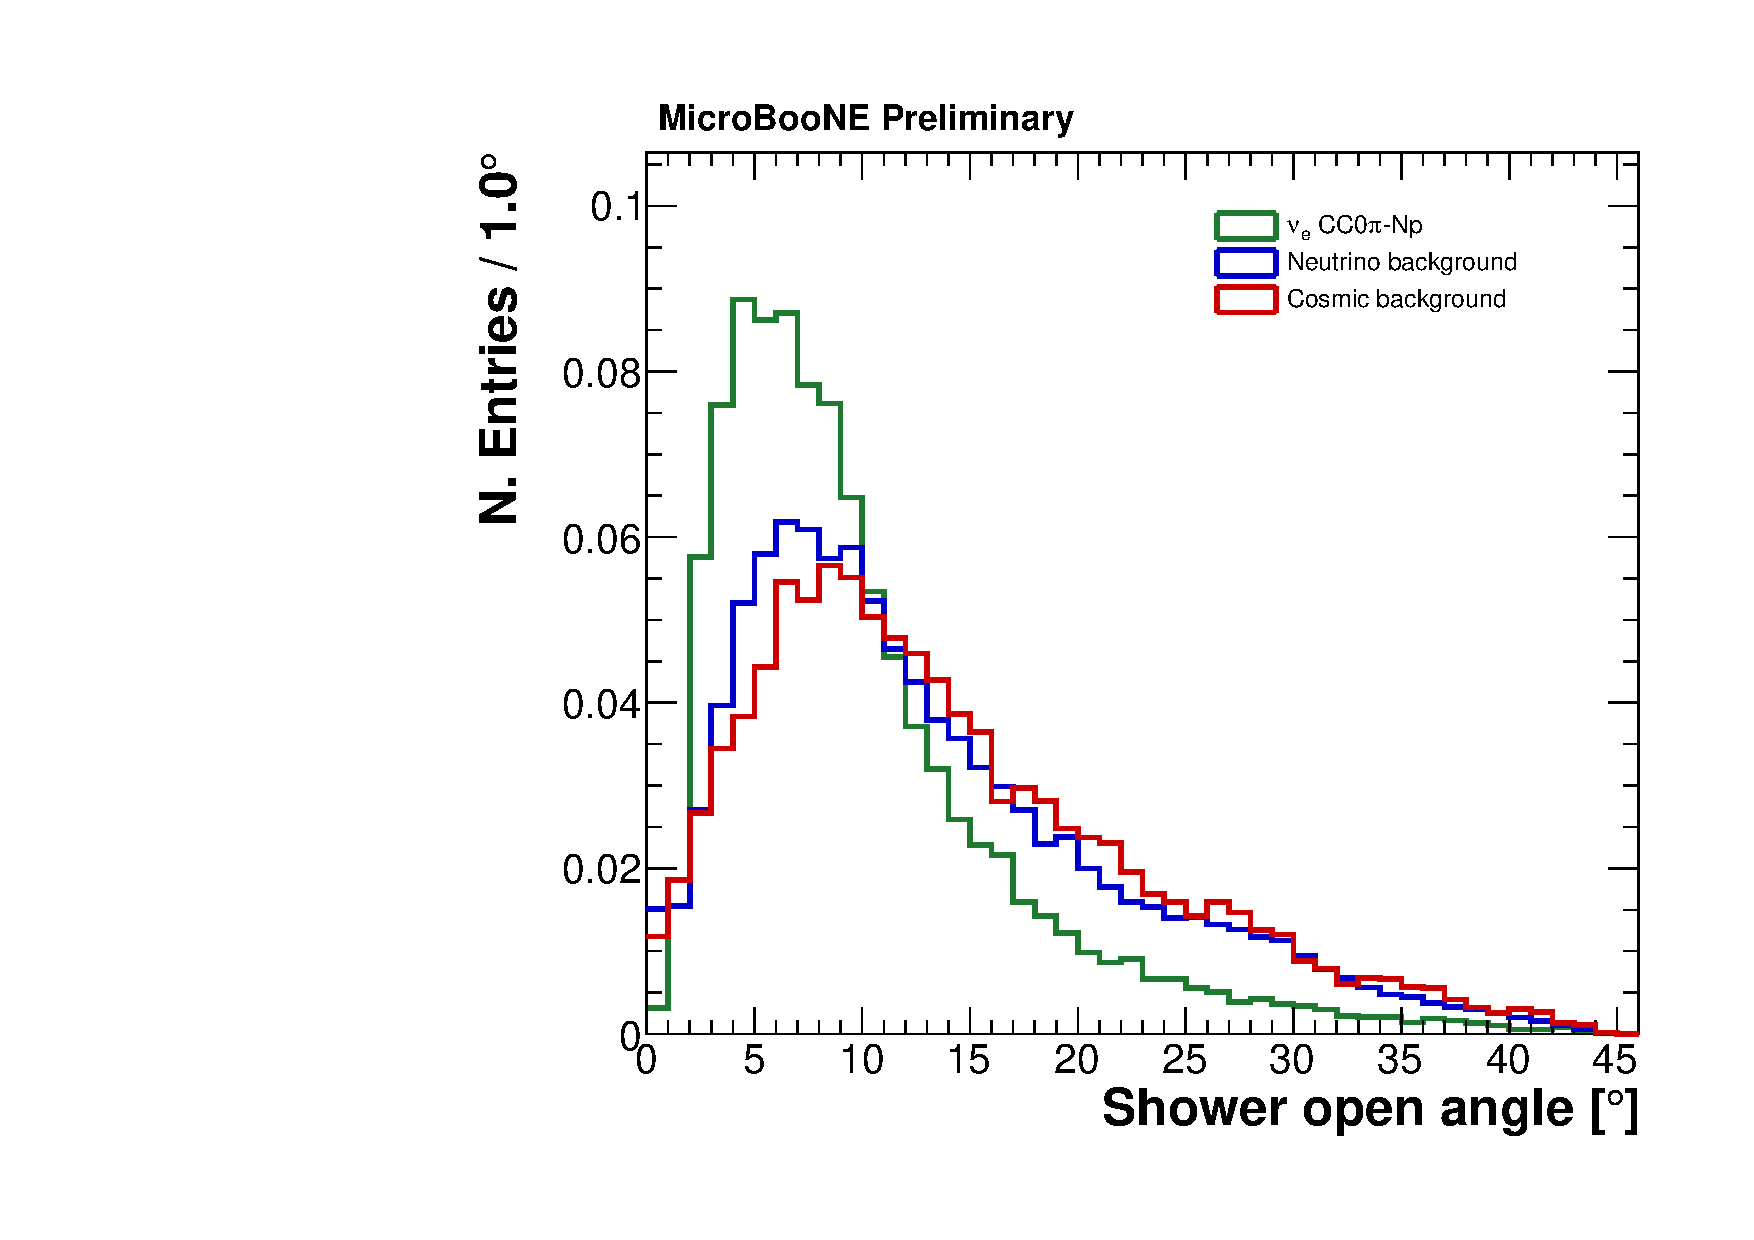
\includegraphics[width=\linewidth]{figures/h_shower_open_angle_norm.pdf}
    \caption{Integral normalized.} \label{fig:open_integral}
  \end{subfigure}
    \begin{subfigure}{0.45\textwidth}
    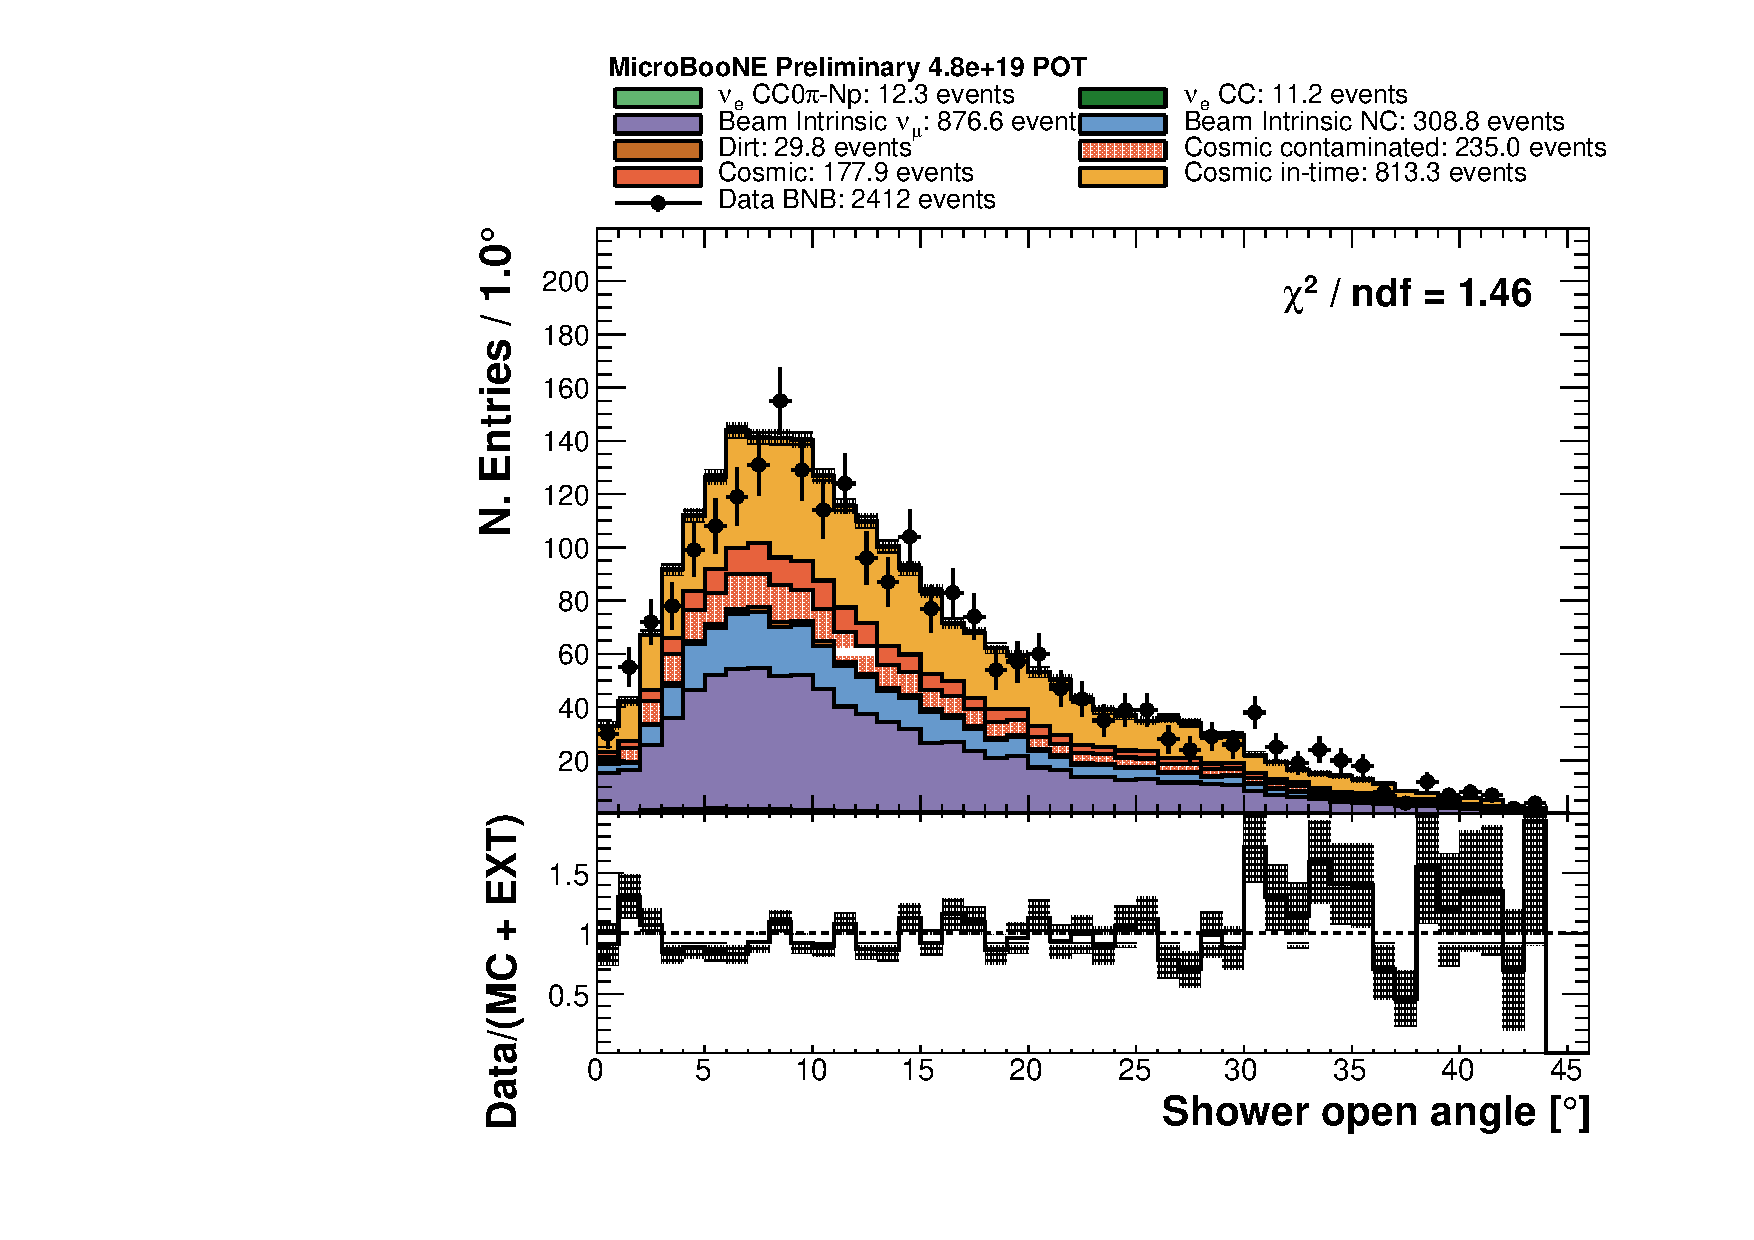
\includegraphics[width=\linewidth]{figures/h_shower_open_angle.pdf}
    \caption{POT normalized.} \label{fig:open_pot}
  \end{subfigure}
  \caption{Integral and POT normalized distributions of the opening angle of the most energetic shower.}
\end{figure}

\item[Most proton-like track length $L < 80~\mathrm{cm}$]. Both neutrino and cosmic background events have on average longer reconstructed tracks than signal events, as shown in \ref{fig:length_norm}. The cut $L < 80~$cm increases the signal purity without significantly decreasing the signal efficiency. The agreement between data and Monte Carlo distributions is good (Figure \ref{fig:length_pot}).

\begin{figure}[htbp]
\centering
  \begin{subfigure}{0.45\textwidth}
    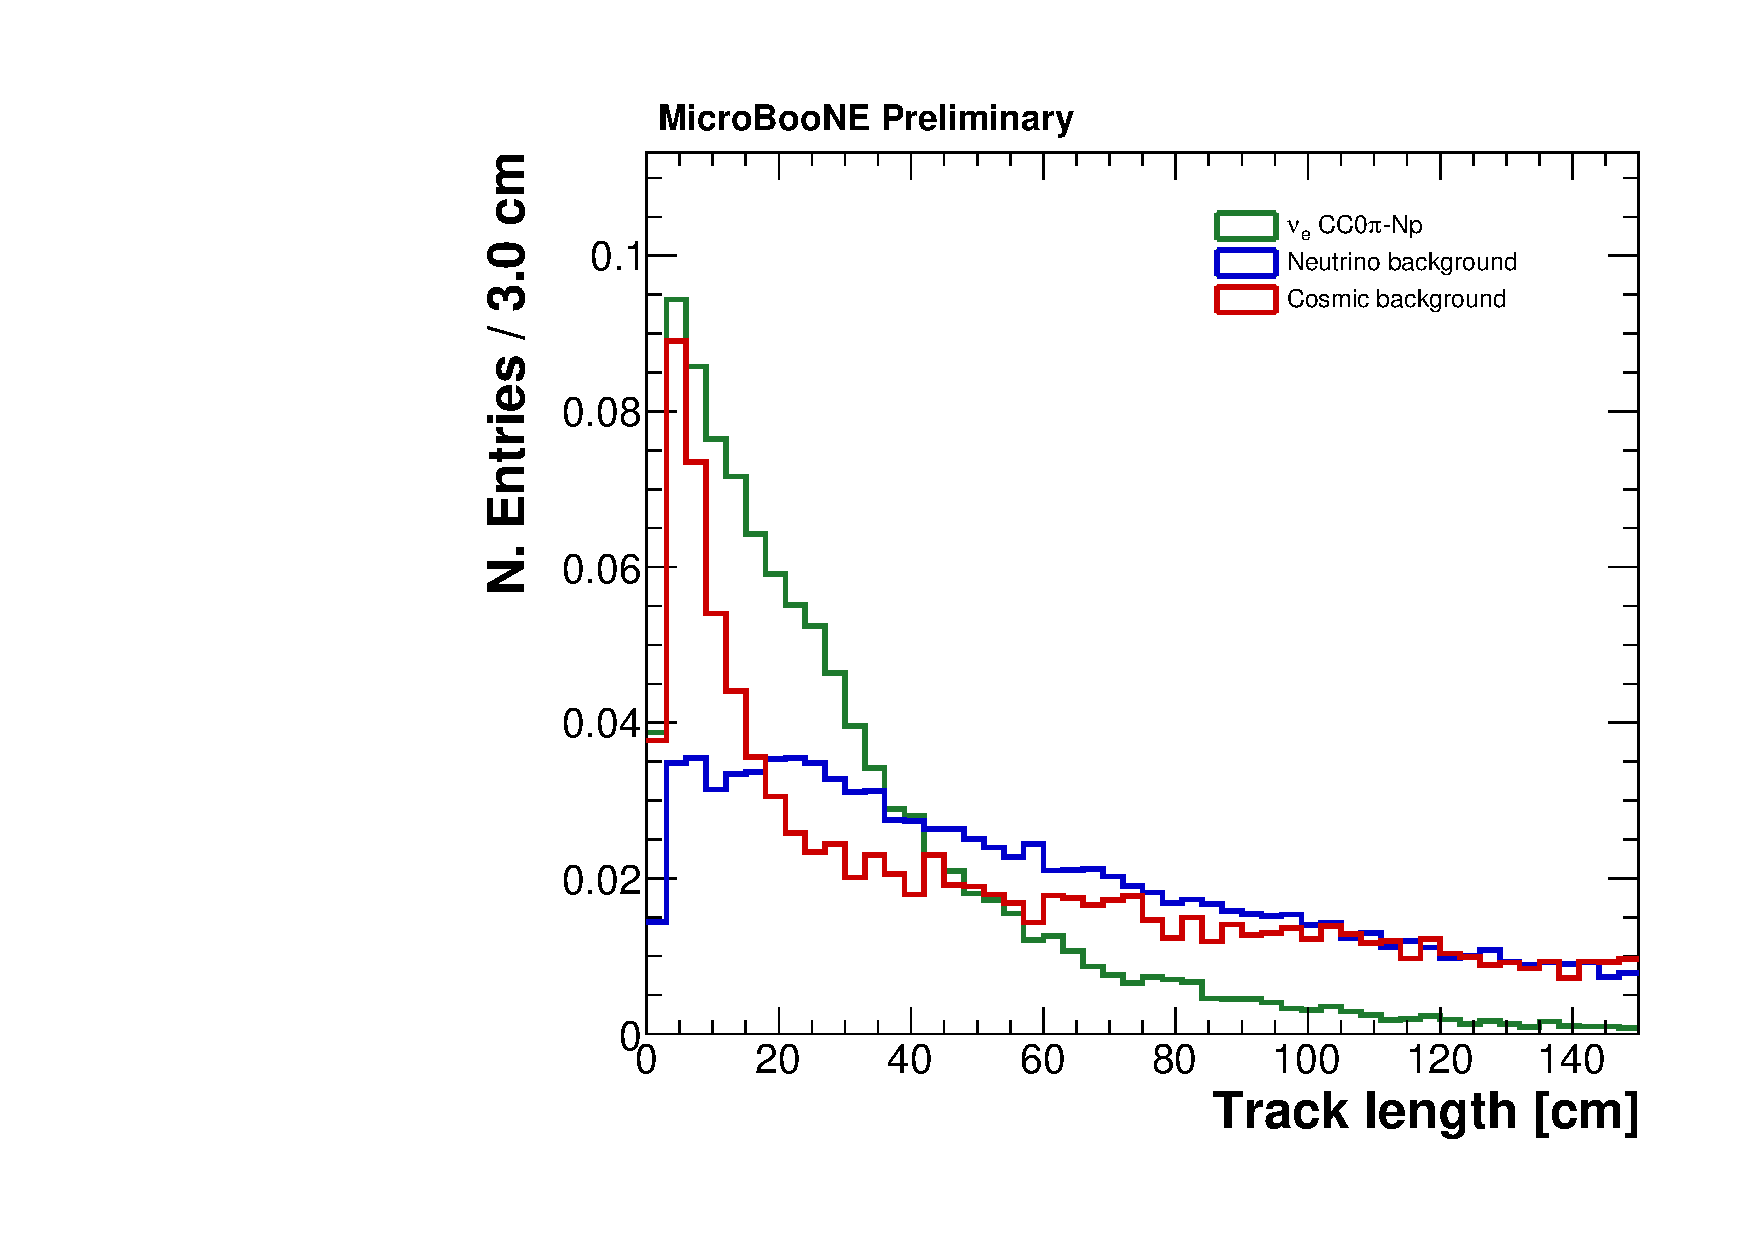
\includegraphics[width=\linewidth]{figures/h_track_length_norm.pdf}
    \caption{Integral normalized.} \label{fig:length_norm}
  \end{subfigure}
    \begin{subfigure}{0.45\textwidth}
    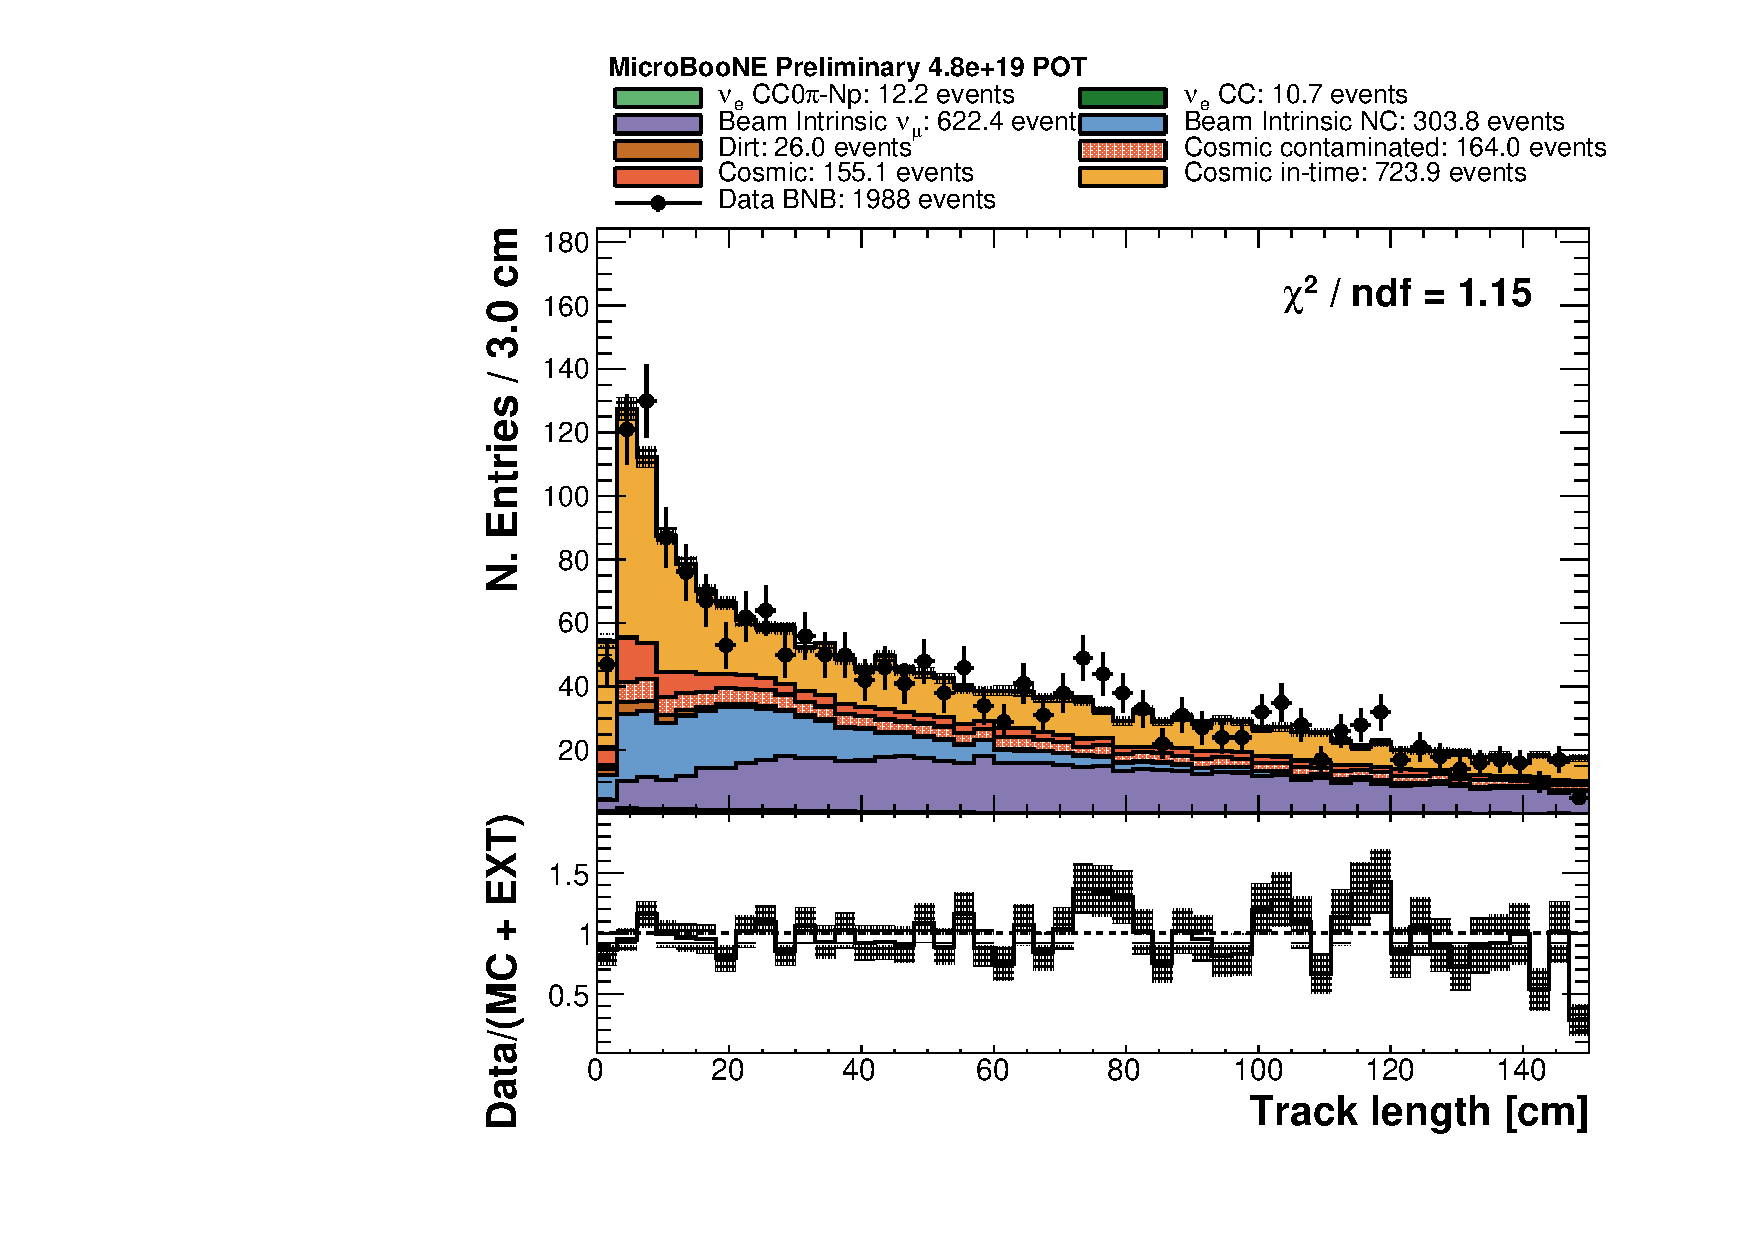
\includegraphics[width=\linewidth]{figures/h_track_length.pdf}
    \caption{POT normalized.} \label{fig:length_pot}
  \end{subfigure}
  \caption{Integral and POT normalized distributions of the length of the most proton-like track.}
\end{figure}

\end{description}

\subsection{Side-bands checks}
\subsubsection{Introduction}
In this section we will show the agreement between data and Monte Carlo for selected samples mostly orthogonal to our $\nu_{e}$ CC0$\pi$-Np signal. In particular, some of the background cuts described in \ref{sec:bkg} will be inverted or removed in order to enhance different background components.

\subsubsection{Photon-enhanced reverse cuts}
It is possible to enhance the neutral-current component (defined as beam intrinsic NC in our analysis) by (1) inverting the cut on the shower $dE/dx$, (2) removing the requirement on the shower opening angle, and (3) removing the cut on the track distance. The $dE/dx$ of the most energetic shower must be within 3.2~MeV/cm and 5~MeV/cm to ensure that the electromagnetic cascade was initiated by a photon. Removing the cut on the shower opening angle allows to include events where two photon showers from a $\pi^{0}\rightarrow 2\gamma$ decay are reconstructed as a single object. The cut on the track distance is removed to increase the size of the sample.
Thus, our final sample will mainly contain NC$\pi^{0}$, with a small contamination of $\nu_{\mu}$ CC$\pi^{0}$ events where the muon track was tagged as a proton-like track.

Figure \ref{fig:photon} shows a good agreement between data and Monte Carlo for the reconstructed energy spectrum of the photon-enhanced event spectrum.

\begin{figure}[htbp]
\centering
  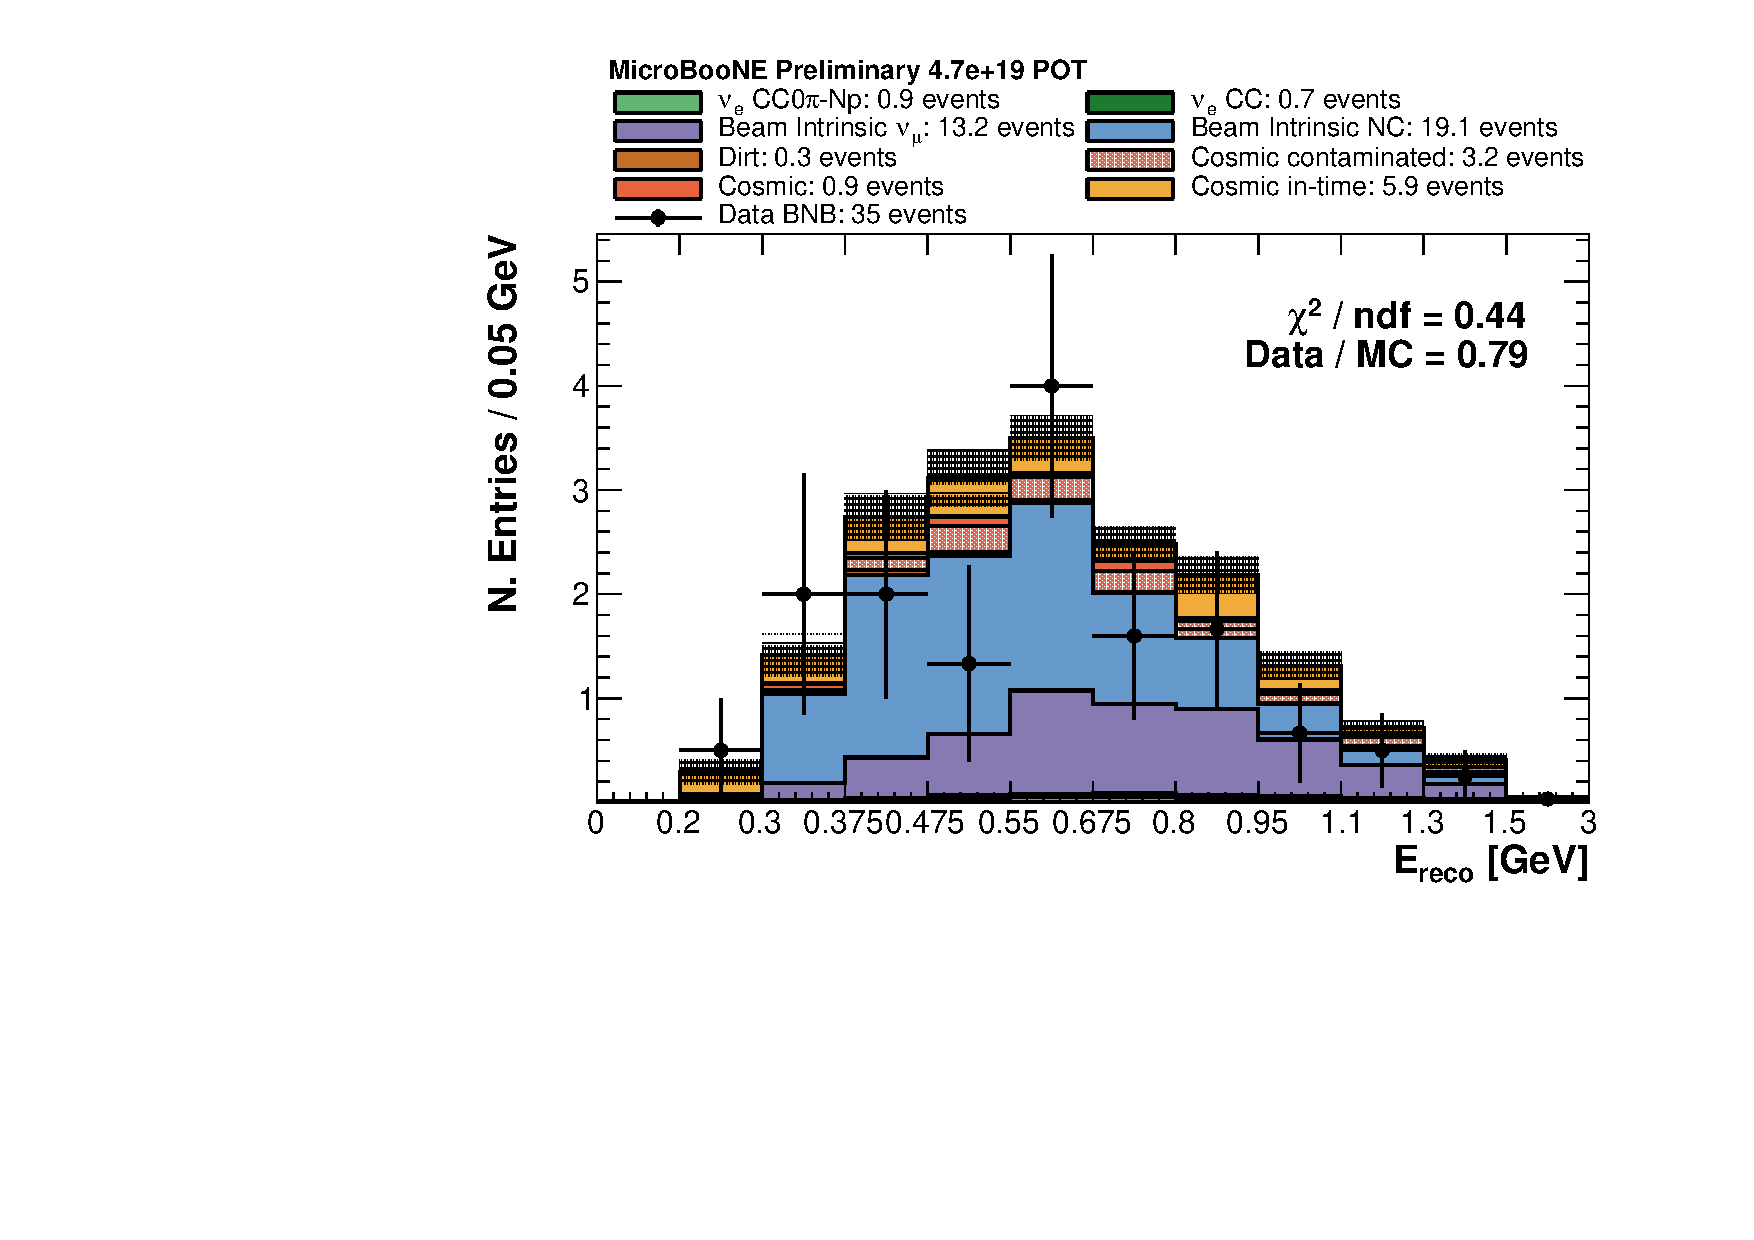
\includegraphics[width=0.65\linewidth]{figures/nc_reco.pdf}
  \caption{Reconstructed energy spectrum of the events selected with the photon-enhanced reverse cuts.}\label{fig:photon}
\end{figure}

\subsubsection{CC \texorpdfstring{$\nu_{\mu}$}{numu}-enhanced reverse cuts}
It is possible to enhance the presence of the CC $\nu_{\mu}$ background (defined as beam intrinsic $\nu_{\mu}$ in our analysis) by (1) requiring a minimum track length, (2) removing the cut on the proton BDT, and (3) requiring that the event is selected by the auxiliary \texttt{UBXSec} module. 
A CC $\nu_{\mu}$ event has, by definition, a muon in the final state: as such, requiring a track length larger than 20~cm and removing the cut on the proton BDT decreases our muon-rejection power. The goal of the auxiliary \texttt{UBXSec} module is to select CC $\nu_{\mu}$ events, so instead of vetoing those events as described in \ref{sec:numu}, we invert this requirement by allowing only the events selected by \texttt{UBXSec}.

Figure \ref{fig:numu_inverted} shows a good agreement between data and Monte Carlo for the reconstructed energy spectrum of the CC $\nu_{\mu}$-enhanced event spectrum.

\begin{figure}[htbp]
\centering
  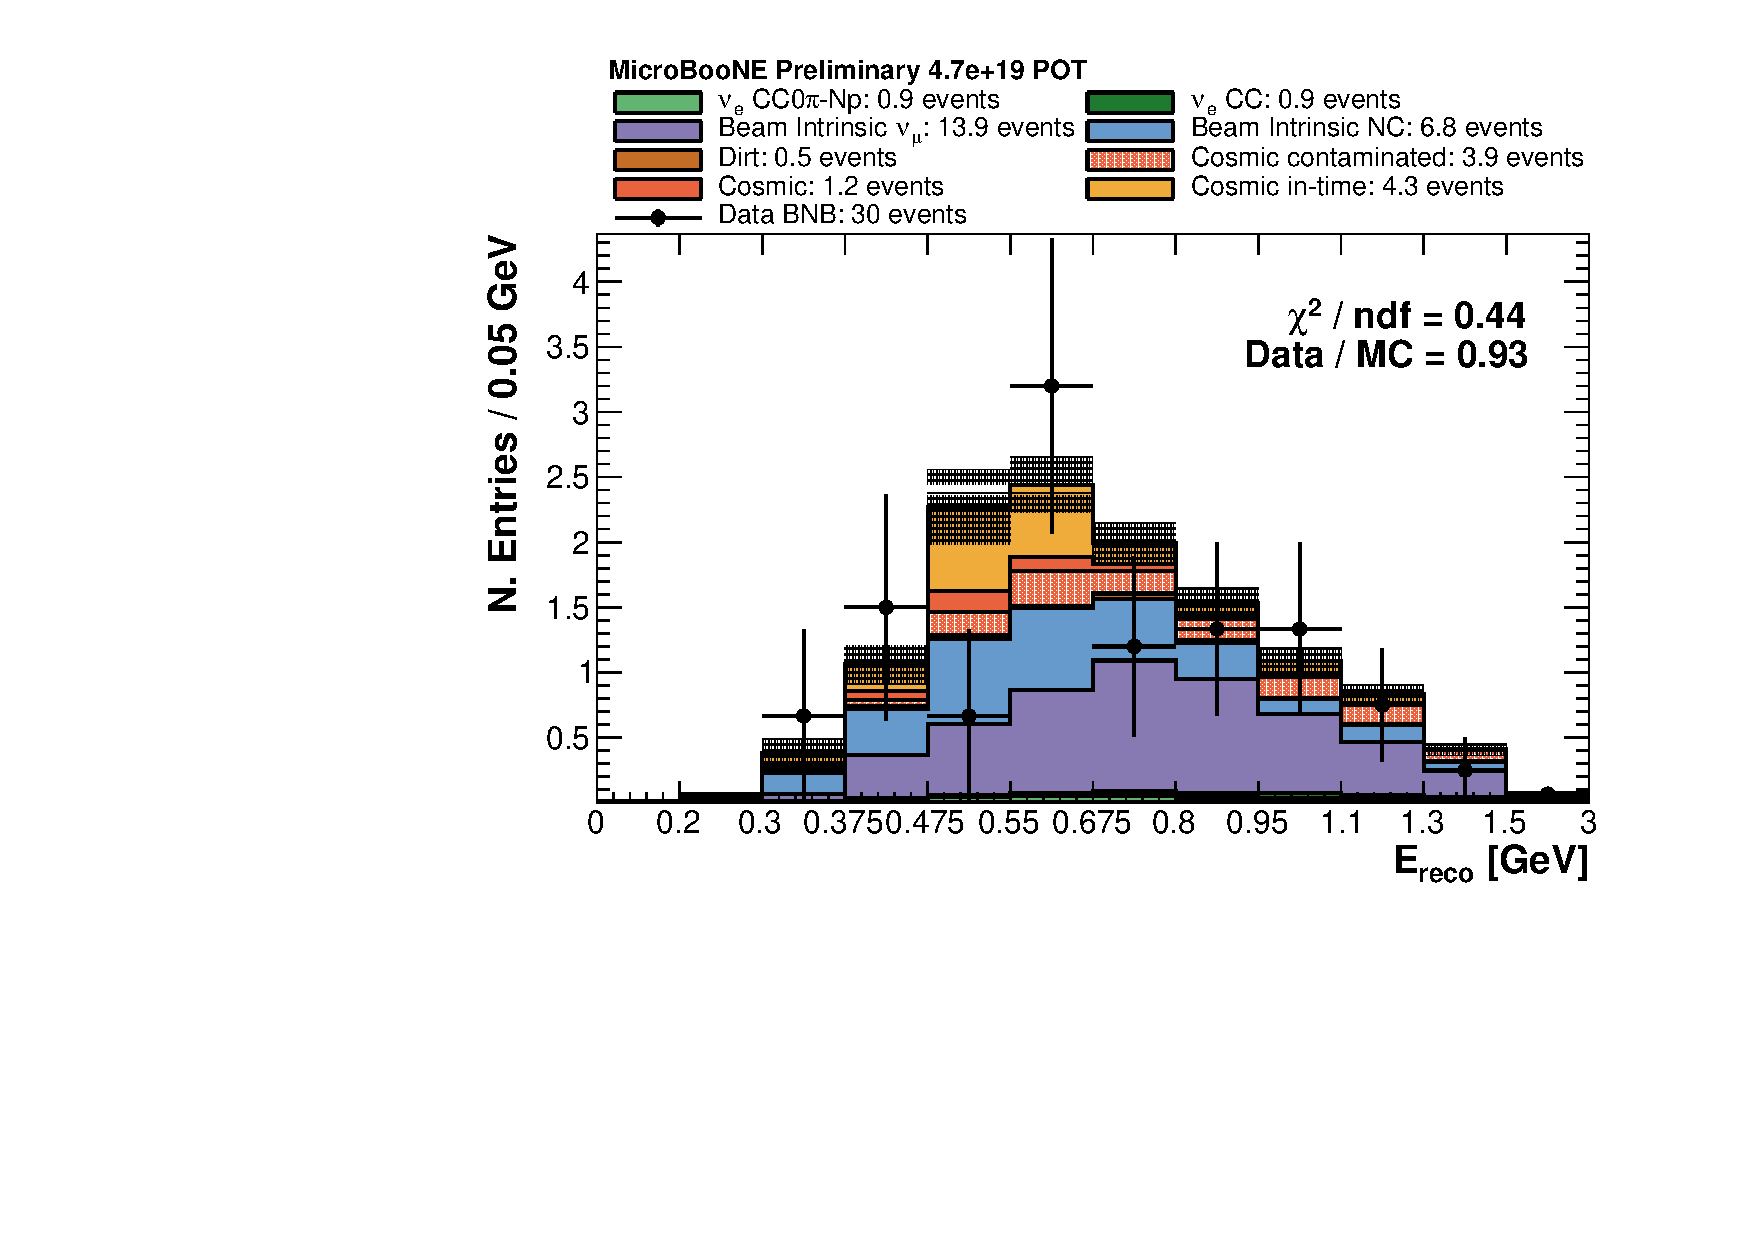
\includegraphics[width=0.65\linewidth]{figures/numu_reco.pdf}
  \caption{Reconstructed energy spectrum of the events selected with the CC $\nu_{\mu}$-enhanced reverse cuts.}\label{fig:numu_inverted}
\end{figure}

\subsection{Future Validation Studies}

\subsubsection{CORSIKA in-time / EXT comparison}
In order to validate the cosmic-ray components of our selected events it is possible to compare simulated events with a CORSIKA cosmic ray producing a flash in the optical system during the beam-gate window and the data EXT sample. 
In this way we will be able to check if the distributions of the variables we use (e.g. shower energy, shower $dE/dx$) have or not a good agreement between the simulation and a well-understood set of data events. 
It will help validating the cosmic background components and also the energy and $dE/dx$ reconstruction procedures.

\subsubsection{Data/MC Comparisons with NuMI}
It is possible to run this analysis on the complementary NuMI dataset. The NuMI neutrino beam has a higher energy than the BNB (the first one is created from 120 GeV protons hitting on a carbon target, while the second one from 8 GeV protons on beryllium). NuMI has also a higher beam intrinsic $\nu_{e}$ component than BNB (5\% vs. 0.5\%), as shown in Figure \ref{fig:numibeam}. Even if off-axis, MicroBooNE will then receive $\sim2500$ $\nu_{e}$ interactions per year. 
As such, a study of the events selected in the NuMI dataset is of fundamental importance to validate the $\nu_{e}$ CC0$\pi$-Np selection algorithm in a different energy region, where the effect of the MiniBooNE low-energy excess should be negligible.

\begin{figure}[htbp]
\centering
  \begin{subfigure}{0.45\textwidth}
    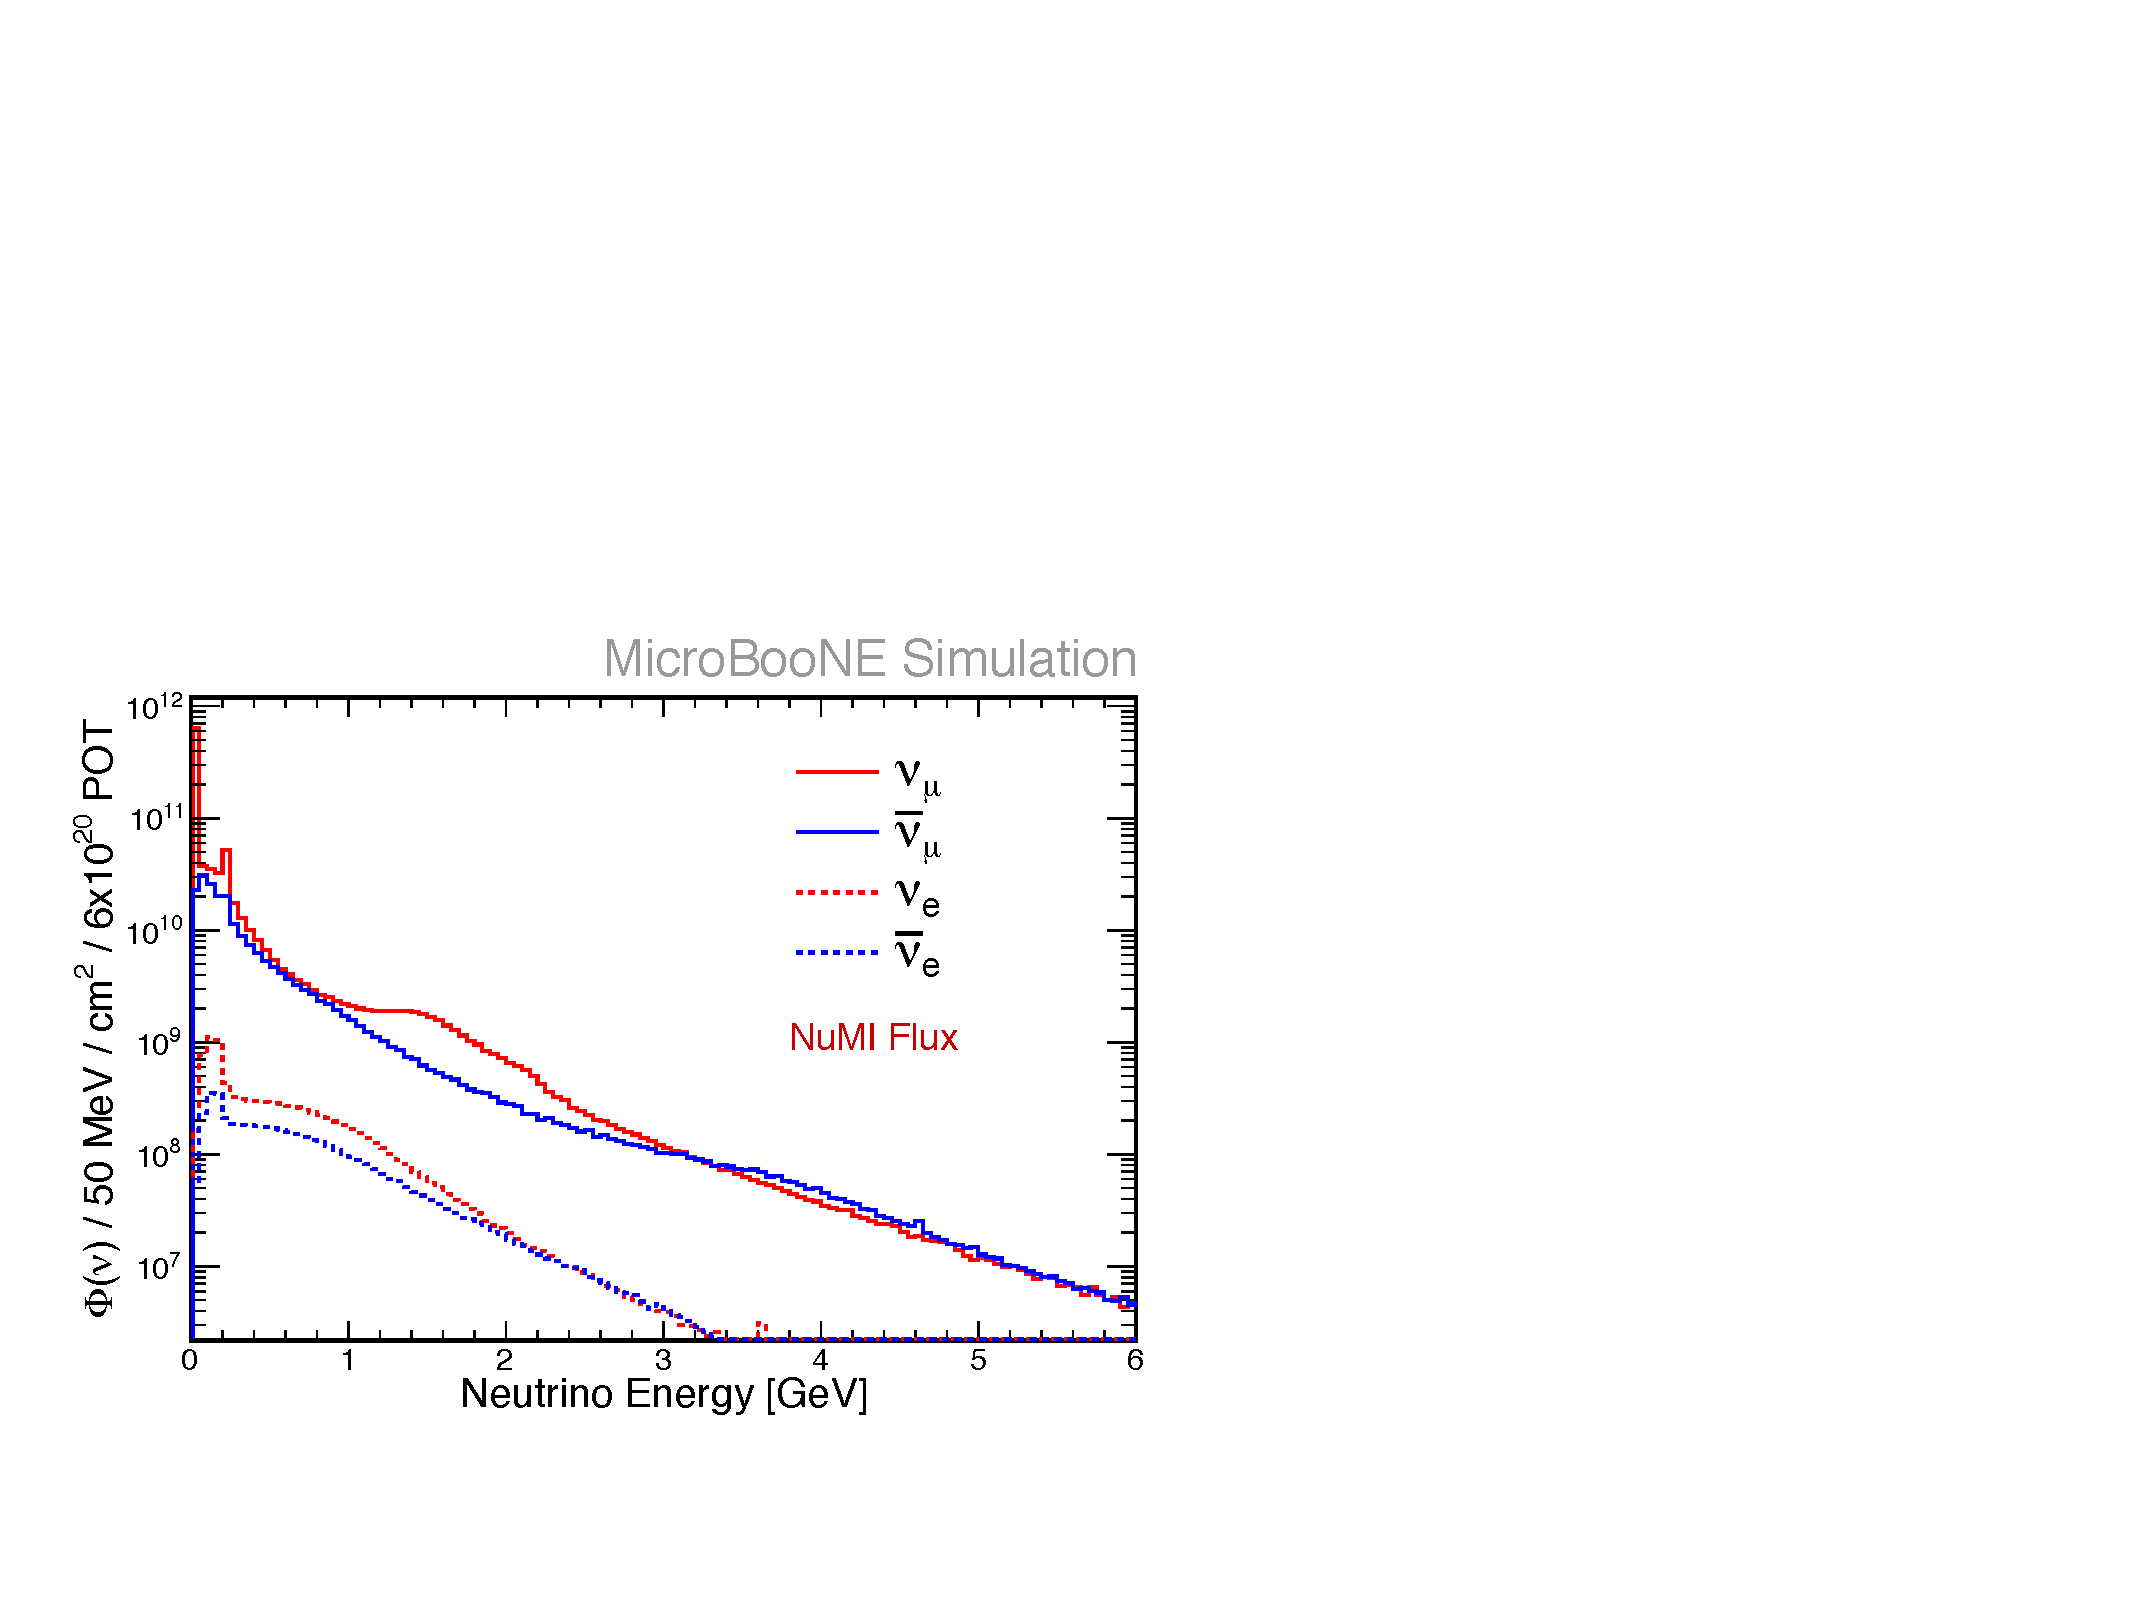
\includegraphics[width=\linewidth]{figures/numi.pdf}
    \caption{NuMI beam flux.} 
  \end{subfigure}
    \begin{subfigure}{0.45\textwidth}
    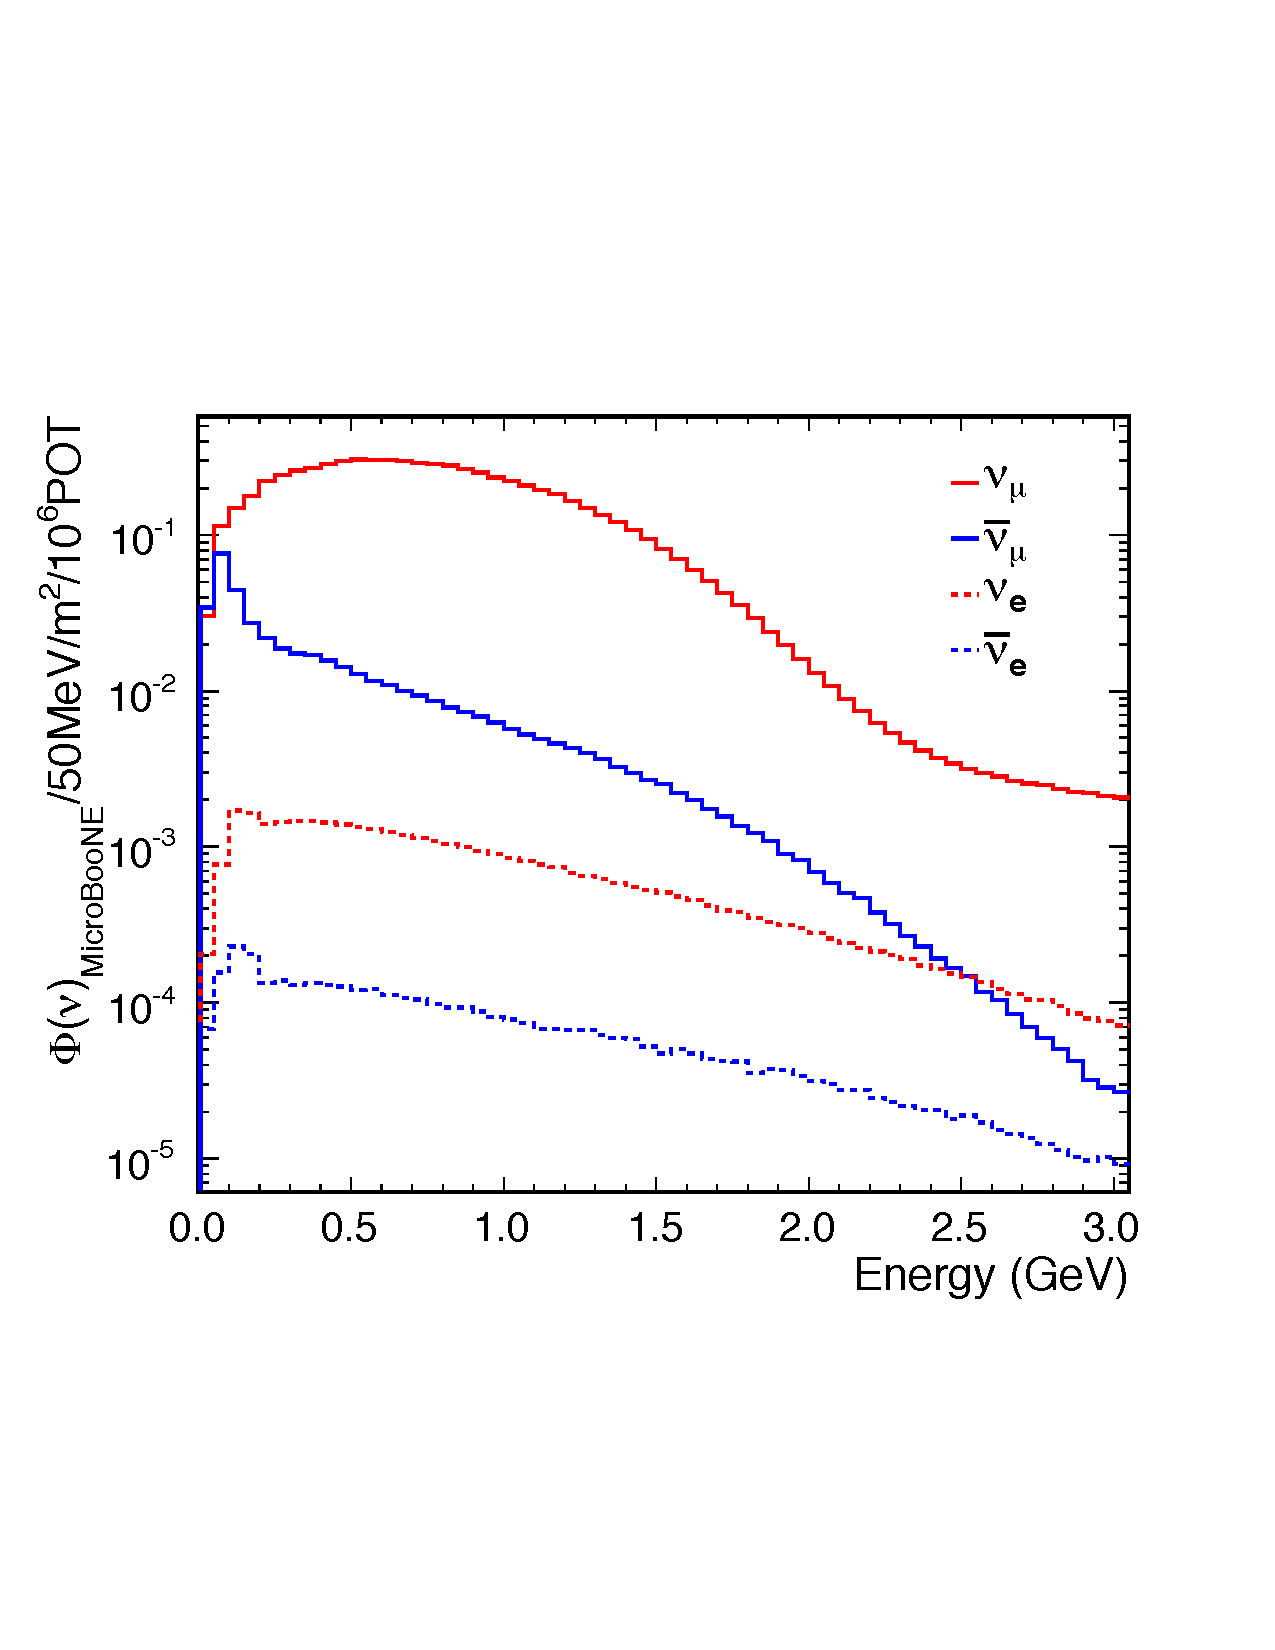
\includegraphics[width=\linewidth]{figures/bnb.pdf}
    \caption{BNB beam flux.} 
  \end{subfigure}
  \caption{NuMI and BNB neutrino fluxes for each neutrino and antineutrino component.}\label{fig:numibeam}
\end{figure}

